% =====================================================================
%  Rosetta — A User's Guide
%
%  Build:  make          (or: pdflatex rosetta-book && pdflatex rosetta-book)
%
%  This is the USER MANUAL. The academic write-up of the same system —
%  its thesis, its evaluation, its related work — is ../../paper/en.
%  Keep the two apart: this book says how to use rosetta, the paper
%  says why it is interesting.
%
%  Package policy: nothing beyond a basic TeX Live install. No
%  tcolorbox, no framed, no titlesec — the callout and code styles
%  below are built from listings, xcolor and plain LaTeX boxes so the
%  book compiles wherever pdflatex does.
% =====================================================================
\documentclass[11pt,a4paper,oneside]{book}

\usepackage[T1]{fontenc}
\usepackage[utf8]{inputenc}
\usepackage[english]{babel}
\usepackage{lmodern}
\usepackage{microtype}
\usepackage[margin=2.7cm,headheight=14pt]{geometry}
\usepackage{booktabs}
\usepackage{longtable}
\usepackage{array}
\usepackage{tabularx}
\usepackage{enumitem}
\usepackage{xcolor}
\usepackage{graphicx}
\usepackage{tikz}
\usetikzlibrary{arrows.meta,positioning,fit,backgrounds,calc}
\usepackage{fancyhdr}
\usepackage{parskip}
\usepackage{caption}
\usepackage{listings}
\usepackage[hidelinks,bookmarksnumbered]{hyperref}

% --- palette ---------------------------------------------------------
\definecolor{rosettablue}{HTML}{1F5C8B}
\definecolor{rosettaorange}{HTML}{C05621}
\definecolor{codebg}{HTML}{F6F6F4}
\definecolor{codeframe}{HTML}{DDDDD8}
\definecolor{kw}{HTML}{1F5C8B}
\definecolor{str}{HTML}{2F6F3E}
\definecolor{cmt}{HTML}{7A7A7A}
\definecolor{notebar}{HTML}{1F5C8B}
\definecolor{warnbar}{HTML}{C05621}

% --- headers ---------------------------------------------------------
\pagestyle{fancy}
\fancyhf{}
\fancyhead[L]{\small\itshape\nouppercase{\leftmark}}
\fancyhead[R]{\small\thepage}
\renewcommand{\headrulewidth}{0.4pt}
\fancypagestyle{plain}{\fancyhf{}\fancyhead[R]{\small\thepage}%
  \renewcommand{\headrulewidth}{0pt}}

% --- inline code -----------------------------------------------------
% \code{} is \texttt: underscores and other specials must be escaped in
% the source (\_). Deliberate — it keeps the macro trivial and the
% compiler catches every miss.
%
% Manifest names are long and full of underscores (compile_definitions,
% cpp26_root, std::shared_ptr<Backend>), and TeX will not break inside a
% typewriter run — so a single name can overrun the margin in a narrow
% table cell. Rebinding \_ inside the group turns every escaped
% underscore into a break opportunity. It is a rebinding rather than a
% catcode change so it works on an argument that was already tokenised,
% which is what happens inside a table cell or another macro.
% \bk adds one by hand, for the paths and :: runs this cannot reach.
\newcommand{\bk}{\discretionary{}{}{}}
\newcommand{\bkus}{\char`\_\bk}
\DeclareRobustCommand{\code}[1]{\texttt{\small\let\_\bkus #1}}
\newcommand{\rosetta}{\textsc{Rosetta}}
\DeclareRobustCommand{\field}[1]{\code{#1}}
\DeclareRobustCommand{\lang}[1]{\code{#1}}

% hyperref re-expands section titles into PDF bookmark strings, where
% \let and font switches are meaningless. Strip the wrappers there and
% keep the text.
\makeatletter
\pdfstringdefDisableCommands{%
  \let\code\@firstofone
  \let\field\@firstofone
  \let\lang\@firstofone
  \let\bk\@empty
  \let\bkus\@empty
  \def\_{\string_}%
  \def\rosetta{Rosetta}%
}
\makeatother

% --- listings --------------------------------------------------------
\lstdefinelanguage{json}{
  morestring=[b]",
  morecomment=[l]{//},
  morecomment=[s]{/*}{*/},
  literate=
   *{:}{{{\color{kw}:}}}{1}
    {[}{{{\color{kw}[}}}{1}
    {]}{{{\color{kw}]}}}{1}
    {\{}{{{\color{kw}\{}}}{1}
    {\}}{{{\color{kw}\}}}}{1},
}

\lstdefinestyle{base}{
  basicstyle=\ttfamily\footnotesize,
  keywordstyle=\color{kw}\bfseries,
  commentstyle=\color{cmt}\itshape,
  stringstyle=\color{str},
  backgroundcolor=\color{codebg},
  frame=single,
  rulecolor=\color{codeframe},
  framesep=5pt,
  xleftmargin=6pt,
  xrightmargin=0pt,
  showstringspaces=false,
  breaklines=true,
  breakatwhitespace=true,
  columns=fullflexible,
  keepspaces=true,
  captionpos=b,
  aboveskip=\medskipamount,
  belowskip=\medskipamount,
}
\lstdefinestyle{cpp}{style=base,language=C++,
  morekeywords={consteval,constexpr,concept,requires,co_await,nullptr,override,final,noexcept}}
% listings ships no JavaScript definition; this is the subset the book uses.
\lstdefinelanguage{javascript}{
  keywords={const,let,var,function,return,new,await,async,class,extends,
            import,export,from,require,if,else,for,of,in,typeof},
  ndkeywords={true,false,null,undefined,this},
  sensitive=true,
  comment=[l]{//},
  morecomment=[s]{/*}{*/},
  morestring=[b]',
  morestring=[b]",
  morestring=[b]`,
}
\lstdefinestyle{js}{style=base,language=javascript}
\lstdefinestyle{py}{style=base,language=Python}
\lstdefinestyle{json}{style=base,language=json}
\lstdefinestyle{sh}{style=base,language=bash,
  keywordstyle=\color{kw},morekeywords={cmake,rosetta_gen,npm,emcmake,jq,python,python3}}
\lstdefinestyle{plain}{style=base,language={}}
\lstset{style=plain}

% --- callouts (no tcolorbox on a basic TeX Live) ----------------------
% A coloured left rule plus an indented block. Built from primitives so
% the book needs nothing beyond the packages above.
\newenvironment{callout}[2]% #1 = bar colour, #2 = label
{\par\medskip\noindent
 \begingroup
 \setlength{\fboxsep}{0pt}%
 \begin{list}{}{\leftmargin=1.2em\rightmargin=0pt\itemindent=0pt\listparindent=0pt
   \topsep=0pt\parsep=\parskip\partopsep=0pt}
 \item[]\hspace*{-1.2em}\makebox[1.2em][l]{\textcolor{#1}{\rule[-0.3ex]{2.2pt}{1.1em}}}%
 \textcolor{#1}{\textbf{\small\MakeUppercase{#2}}}\par\nopagebreak\smallskip}
{\end{list}\endgroup\par\medskip}

\newenvironment{note}{\begin{callout}{notebar}{note}}{\end{callout}}
\newenvironment{warn}{\begin{callout}{warnbar}{watch out}}{\end{callout}}

% --- table helpers ---------------------------------------------------
\newcolumntype{L}[1]{>{\raggedright\arraybackslash}p{#1}}
\newcolumntype{C}[1]{>{\centering\arraybackslash}p{#1}}
\newcommand{\yes}{\textcolor{str}{\textbf{yes}}}
\newcommand{\no}{\textcolor{warnbar}{\textbf{no}}}
\newcommand{\req}{$\bullet$}

% --- line breaking ---------------------------------------------------
% Belt and braces for the long typewriter runs \code's own break
% opportunities cannot reach: let TeX stretch a line a little rather
% than overrun the margin.
\tolerance=1200
\emergencystretch=2.5em

% --- misc ------------------------------------------------------------
\setlist[itemize]{itemsep=2pt,topsep=4pt,parsep=0pt}
\setlist[enumerate]{itemsep=2pt,topsep=4pt,parsep=0pt}
\setcounter{tocdepth}{1}
\setcounter{secnumdepth}{2}
\captionsetup{font=small,labelfont=bf}

% --- title page ------------------------------------------------------
% The logo lives with the rest of the repository's media rather than in
% this directory. Spelled as one path rather than through \graphicspath
% because \IfFileExists does NOT consult graphicspath — it would have
% found nothing and silently skipped the logo. The guard keeps the book
% buildable from a copy of docs/book alone: a missing logo leaves a gap,
% not a failed run.
\newcommand{\logopath}{../../media/logo-rosetta.png}

\hypersetup{pdftitle={Rosetta — A User's Guide},
            pdfauthor={Frantz Maerten},
            pdfsubject={Multi-language bindings for unmodified C++ with C++26 reflection}}

% =====================================================================
\begin{document}

\frontmatter

\begin{titlepage}
\centering
\vspace*{1.2cm}

{\Huge\bfseries\rosetta\par}
\vspace{0.5cm}
{\LARGE A User's Guide\par}
\vspace{0.7cm}
{\large Multi-language bindings for unmodified C++,\\
        generated once with C++26 static reflection\par}

% \vfill on both sides so the logo sits centred in whatever space the
% title and author blocks leave, rather than hard against the title.
\vfill
\IfFileExists{\logopath}{%
  \includegraphics[width=0.66\textwidth]{\logopath}%
}{}
\vfill

{\large Frantz Maerten\par}
\vspace{0.2cm}
{\small\texttt{fmaerten@gmail.com}\par}
\vspace{1.0cm}
{\small\today\par}
\end{titlepage}

\chapter*{Preface}
\addcontentsline{toc}{chapter}{Preface}
\markboth{Preface}{Preface}

This book is about a single, narrow claim: that the information needed to
expose a C++ library to Python, to JavaScript, to Lua, to a REST endpoint or
to a property panel is \emph{already in the header}, and that a compiler can
be made to read it out.

Everything else follows from taking that claim seriously. You do not write a
binding. You write down \emph{what} you want bound --- a list of headers and a
list of target languages --- and a program compiled against your types answers
the rest by reflection. Your class definitions never change.

\section*{Who this is for}

You have a C++ library. You want it callable from somewhere else, ideally from
several somewheres, and you would rather not maintain a hand-written wrapper
per destination. You are comfortable with CMake and with your own build.

You do \emph{not} need to know anything about C++26 static reflection to use
rosetta. Reflection is what makes the tool possible, and Chapter~\ref{ch:pipeline}
explains where it runs and why the pipeline has the shape it does --- but the
surface you work with is a JSON file and a command-line tool.

\section*{How to read it}

\begin{description}[leftmargin=1.4cm,style=nextline,font=\normalfont\itshape]
  \item[In a hurry] Chapter~\ref{ch:first} is a complete first binding, from an
    unmodified header to an importable Python module. Read that, then come back.
  \item[Evaluating rosetta] Chapters~\ref{ch:what} and~\ref{ch:pipeline} say what
    the system does and what it costs, including the parts that do not work.
  \item[Using it in earnest] Part~II is the manifest, field by field, and is the
    part you will return to. Part~IV is the tool that consumes it.
  \item[Documenting what you bind] Part~III is the two ways metadata reaches a
    binding: annotations you write, and the Doxygen comments and default
    arguments your headers already carry
    (chapter~\ref{ch:documentation}, on by default).
  \item[Pushing past bindings] Part~V covers the runtime object model, scripting
    the metadata itself, and writing a backend of your own.
\end{description}

The appendices are lookup tables: every manifest field, every annotation, every
target, and the errors you are most likely to hit.

\section*{Conventions}

\code{Monospace} is a literal --- a field name, a path, a command. A
\emph{manifest} always means the \code{manifest.json} driving one binding
project. \emph{Generation host} is the machine that runs the reflection
compiler; \emph{target} is wherever the generated binding is finally built,
which is deliberately not the same machine.

Two callouts appear throughout:

\begin{note}
Something worth knowing that is not on the shortest path.
\end{note}

\begin{warn}
Something that will cost you an afternoon if you meet it unprepared.
\end{warn}

\section*{Status}

Rosetta is a prototype, and this book says so where it matters. It tracks
in-flight C++ proposals --- P2996 (reflection), P3394 (annotations), P3294
(token injection) --- and is developed against the Bloomberg
\code{clang-p2996} fork, which is currently the only front-end that carries
all of what it uses. What the tool \emph{generates} has no such constraint:
that is the whole point, and Chapter~\ref{ch:pipeline} is where the distinction
is made precise.

\section*{Related documents}

The repository carries the reference material this book is built from ---
\code{docs/MANIFEST.md}, \code{docs/ROSETTA\_GEN.md},
\code{docs/ANNOTATIONS.md}, \code{docs/COVERAGE.md} and the rest. Where a
detail here is compressed, those are the long form. The academic write-up of
the same system, with its evaluation and its related work, lives under
\code{paper/}; it argues that reflection can serve as an interface description
language, where this book simply assumes it and gets on with the job.


\tableofcontents

\mainmatter

\part{Understanding rosetta}
\input{ch/01-what-is-rosetta}
\chapter{The pipeline, and why it has that shape}
\label{ch:pipeline}

Binding a library with rosetta is a \emph{pipeline} rather than a single
command. That is not an implementation choice --- it is the only shape the
problem admits. This chapter explains why, because almost every surprise in
later chapters resolves back to it.

\section{The constraint everything follows from}

C++26 reflection answers questions \textbf{at the compile time of a program
that includes your headers}. It cannot be queried from a script, from a
configuration file, or from a build system. Only from C++, being compiled, with
your types in scope.

So to learn the shape of your types, something has to \textbf{compile}. To turn
those answers into files on disk, that something has to \textbf{run}.

\begin{center}
\emph{Compile, then run.} Everything below is that sequence, plus one step
before it and one after.
\end{center}

\section{The five steps}

\begin{center}
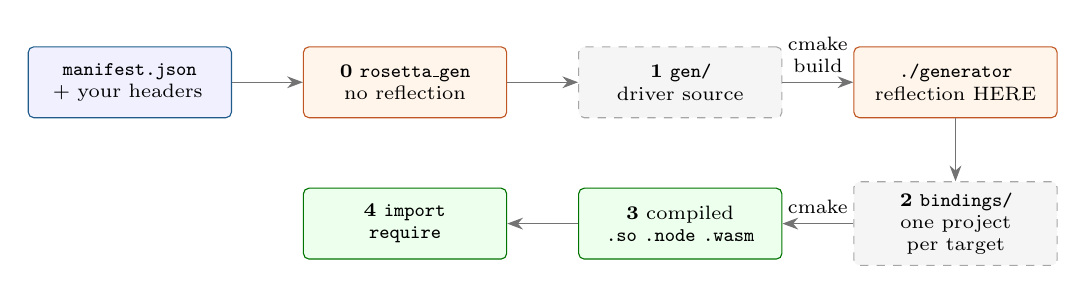
\begin{tikzpicture}[
  node distance=5mm,
  b/.style={draw,rounded corners=2pt,align=center,font=\scriptsize,inner sep=4pt,text width=23mm,minimum height=9mm},
  user/.style={b,fill=blue!6,draw=rosettablue},
  tool/.style={b,fill=orange!8,draw=rosettaorange},
  gen/.style={b,fill=black!4,draw=black!35,dashed},
  fin/.style={b,fill=green!7,draw=green!45!black},
  arr/.style={-{Stealth[length=2mm]},draw=black!55,font=\scriptsize}
]
\node[user] (m) {\texttt{manifest.json}\\+ your headers};
\node[tool,right=9mm of m] (rg) {\textbf{0}\ \texttt{rosetta\_gen}\\\scriptsize no reflection};
\node[gen,right=9mm of rg] (g) {\textbf{1}\ \texttt{gen/}\\driver source};
\node[tool,right=9mm of g] (drv) {\texttt{./generator}\\\scriptsize reflection HERE};
\node[gen,below=8mm of drv] (bind) {\textbf{2}\ \texttt{bindings/}\\one project per target};
\node[fin,left=9mm of bind] (built) {\textbf{3}\ compiled\\\texttt{.so .node .wasm}};
\node[fin,left=9mm of built] (load) {\textbf{4}\ \texttt{import}\\\texttt{require}};
\draw[arr] (m) -- (rg);
\draw[arr] (rg) -- (g);
\draw[arr] (g) -- node[above,align=center]{cmake\\build} (drv);
\draw[arr] (drv) -- (bind);
\draw[arr] (bind) -- node[above]{cmake} (built);
\draw[arr] (built) -- (load);
\end{tikzpicture}
\end{center}

\subsection*{Step 0 --- build \code{rosetta\_gen}}

\code{rosetta\_gen} is a JSON-to-C++ text templater. It does no reflection at
all and builds with an off-the-shelf C++17 compiler. You build it once.

It exists so that what \emph{you} write is a manifest and not a driver program.
Given \code{manifest.json} it emits three files: a \code{<name>.cpp} containing
a \code{main()} that reflects, a \code{bindings.h} with your types (and any
out-of-line annotations) baked in, and a \code{CMakeLists.txt} that knows where
the reflection toolchain lives.

\emph{Your library:} untouched. \code{rosetta\_gen} never opens your headers.
It only copies their names into the driver it writes.

\subsection*{Step 1 --- compile and run the driver}

Three commands, because ``compile then run'' is three things --- emit the
program, build it, execute it:

\begin{lstlisting}[style=sh]
rosetta_gen manifest.json gen     # emit the driver source
cmake -S gen -B gen/build         # COMPILE it -- reflection happens HERE
cmake --build gen/build
./generator bindings              # RUN it -- writes one project per target
\end{lstlisting}

During the \emph{compile}, clang-p2996 evaluates the reflection operators in
the driver: it walks your classes, enumerates fields and methods, reads
annotations, and resolves each member against the target language's type gate.
\textbf{Every decision about what can and cannot be bound is made at this
moment.} During the \emph{run}, the driver does nothing clever --- it prints
the conclusions it was compiled with.

Neither half can be skipped. A compiler cannot write your binding files; a
program cannot see types it was not compiled against.

\emph{Your library:} read for the \textbf{first} time, as source, by the C++26
toolchain.

\subsection*{Step 2 --- what lands in \code{bindings/}}

One self-contained project per target, plus \code{coverage.json} --- a
machine-readable account of what bound and what did not, available
\emph{before} anything is compiled.

The generated code is fully expanded (Section~\ref{sec:reflection-free}). No
splices, no \code{<experimental/meta>}, nothing that needs the fork.

\subsection*{Step 3 --- compile a backend}

Ordinary CMake, or npm, or emcmake, over an ordinary C++ project.

\emph{Your library:} read a \textbf{second} time --- the generated binding
\code{\#include}s your headers and calls your functions. This is where
\field{user\_sources} are compiled and \field{user\_lib} is linked in.

\subsection*{Step 4 --- load it}

\code{import}, \code{require}, \code{dlopen}. Nothing rosetta-specific is left.

\section{Your library is read three times, for different reasons}

\begin{center}
\begin{tabular}{@{}llll@{}}
\toprule
\textbf{Pass} & \textbf{By} & \textbf{To} & \textbf{Needs C++26} \\
\midrule
step 0 & \code{rosetta\_gen}       & \textbf{read} your comments  & \no \\
step 1 & the reflection driver  & \textbf{describe} your types & \yes \\
step 3 & the generated binding  & \textbf{call} them           & \no \\
\bottomrule
\end{tabular}
\end{center}

The middle row is the single most useful thing to hold in your head. The first
is the odd one out and worth a sentence: comments are not reflectable --- P2996
describes declarations, not the text around them --- so the documentation your
headers already carry is read \emph{lexically}, by the tool, while it is
emitting the driver. That pass compiles nothing and needs no toolchain; what it
finds is matched against what step~1 reflects, and dropped where the two
disagree. Chapter~\ref{ch:documentation} is about that pass.

The table has one further consequence worth stating on its own:

\begin{warn}
Annotations written \textbf{inline} --- \code{[[= rosetta::doc\{\ldots\} ]]} ---
pull \code{<experimental/meta>} into your header. Pass~2 then needs the C++26
toolchain as well, and the ``no reflection on the target'' promise is lost.
Out-of-line annotations (a \code{.ann.json} side-car) keep your header plain
C++ and pass~2 reflection-free. See Section~\ref{sec:outofline}.
\end{warn}

\section{Two commands, not five}

You rarely run the steps by hand. \code{rosetta\_gen --build} chains all of
them:

\begin{lstlisting}[style=sh]
rosetta_gen --build manifest.json
\end{lstlisting}

It emits \code{gen/}, builds and runs the driver, and then compiles every
backend the manifest declares --- each with its own build shape (plain
\code{cmake}, \code{npm install} + \code{npm run build}, \code{emcmake}, a
second-stage \code{dotnet build} or \code{mvn package}). A backend whose
toolchain is missing is \emph{skipped with a note}, not an error, and every run
ends with a per-backend summary.

\code{rosetta\_gen --clean manifest.json} takes you back to sources. Chapter~\ref{ch:rosettagen}
is the full reference for both.

The manual sequence remains useful for exactly the reasons you would expect:
inspecting \code{bindings.h}, hacking on the emitted driver, or wiring the
stages into a build system of your own.

\section{When to re-run what}

The two-pass structure decides this, and getting it wrong is the most common
way to be confused by rosetta.

\begin{center}
\small
\begin{tabular}{@{}L{6.2cm}L{7.4cm}@{}}
\toprule
\textbf{What changed} & \textbf{What to do} \\
\midrule
A field or method: added, removed, retyped &
  Rebuild the backend. The generated binding is expanded, so this needs a
  regeneration \emph{if the member set changed} --- re-run \code{--build}. \\
\addlinespace
An \textbf{inline} annotation &
  Re-run \code{--build}: the annotation is read during pass~1. \\
\addlinespace
A \textbf{side-car} \code{.ann.json} &
  Re-run \code{rosetta\_gen} \emph{and} the generator, not just the binding
  build --- the JSON is baked into \code{bindings.h} at \code{rosetta\_gen}
  time. \\
\addlinespace
A class added, or \field{targets} changed &
  Re-run the whole pipeline. \\
\addlinespace
A \field{user\_sources} glob now matches new files &
  Re-run \code{rosetta\_gen}: globs expand at generation time. \\
\addlinespace
The manifest moved &
  Re-run. Every relative path in it resolves from the manifest's own directory. \\
\bottomrule
\end{tabular}
\end{center}

\begin{note}
Re-emitting is idempotent: unchanged files are not rewritten, so the next
\code{cmake --build} recompiles nothing. Running the pipeline again when you
are not sure is cheap.
\end{note}

\section{The footgun the tool warns about}

If the emitted sources changed but a \code{generator} binary from a previous
emit still sits next to the output directory, running it without rebuilding
\textbf{silently re-emits the old bindings}. The tool detects this and prints a
rebuild note. Believe it.

The related one: a fresh checkout (or a \code{--clean}) leaves
\code{out\_dir/build} unconfigured, so \code{cmake --build} alone fails. The
\emph{configure} step is printed as a \code{next:} hint when that happens.

\chapter{Your first binding}
\label{ch:first}

This chapter goes from an unmodified header to an importable Python module and
a loadable Node addon. It is deliberately complete: every command, in order,
with what each one produces.

\section{Prerequisites}

\begin{itemize}
  \item A \textbf{clang-p2996} build. Rosetta looks for it at
    \code{\$ENV\{HOME\}/devs/c++/clang-p2996/build} by default; anywhere else
    is fine, you just say where (Section~\ref{sec:toolchain-paths}).
  \item \textbf{CMake} 3.28 or later, and Ninja or Make.
  \item For the Python target, \code{pip install pybind11}. For Node,
    \code{npm}. For WebAssembly, an activated emsdk.
\end{itemize}

The reflection flags rosetta's generated projects use, should you need to know
them: \code{-freflection -freflection-latest -fexperimental-library}, plus
\code{-fannotation-attributes} for anything using annotations.

\begin{note}
Only the \emph{generation host} needs the fork. Everything under
\code{bindings/} builds with a stock compiler --- with the two documented
exceptions, \lang{rest} and \lang{json}.
\end{note}

\section{The whole build, in two commands}
\label{sec:twocommands}

Everything in this chapter reduces to two lines. Scaffold a binding project
next to your library with \code{tools/rosetta\_init.py} --- it writes a
\code{manifest.json} skeleton and a bootstrap \code{CMakeLists.txt} --- and
then:

\begin{lstlisting}[style=sh]
# 1. one-time bootstrap: fetch rosetta into extern/ and build rosetta_gen
cmake -B build && cmake --build build -j10

# 2. generate the generator, run it, and compile every target
./extern/rosetta/bin/rosetta_gen --build manifest.json -j10
\end{lstlisting}

That is the whole pipeline. The rest of this chapter takes the two apart.

\subsection*{What the first command does}

The bootstrap \code{CMakeLists.txt} fetches rosetta into \code{extern/} (an
existing checkout is left alone) and builds the \code{rosetta\_gen} tool. The
binary always lands in \code{<rosetta>/bin/rosetta\_gen} --- not in the build
tree --- so from your project it is \code{./extern/rosetta/bin/rosetta\_gen}.

This step needs \textbf{no reflection}: \code{rosetta\_gen} is a JSON reader
and a text templater, and builds with an off-the-shelf C++17 compiler. It is
also the only one you run once --- nothing below re-runs it.

\subsection*{What the second command does}

\code{--build} chains the three stages of Chapter~\ref{ch:pipeline}: it emits
the generator project into \code{gen/}, builds it (\textbf{this} is the step
that needs clang-p2996, and where reflection runs), runs it to write one
project per target into \code{bindings/}, and then compiles each of those.

\begin{note}
\code{-j10} is passed to \emph{every} CMake build the command drives --- the
generator's and each backend's. A bare \code{-j} means one job per core.
Backends are still built one after another, so this parallelises within a
backend, not across them; \code{--only python,node} is how you cut the matrix
while iterating (Section~\ref{sec:onlyskip}).
\end{note}

\subsection*{Inside the rosetta repository instead}

If you are working in a checkout of rosetta itself rather than a scaffolded
project, there is no bootstrap to run --- build the tool directly:

\begin{lstlisting}[style=sh]
cmake -G Ninja -S tools/rosetta_gen -B tools/rosetta_gen/build
cmake --build tools/rosetta_gen/build -j10
\end{lstlisting}

The binary lands in the same place, \code{<repo>/bin/rosetta\_gen}. This is the
form the examples in \code{examples/} use.

\section{The library --- leave it alone}

\begin{lstlisting}[style=cpp]
// my_lib/person.h
#pragma once
#include <string>

struct Person {
    std::string name;
    int         age = 0;
    std::string id;

    Person() = default;
    Person(std::string n, int a) : name(std::move(n)), age(a) {}

    std::string greet(const std::string &salutation) const;
};
\end{lstlisting}

Note what is \emph{not} there: no macro, no registration call, no rosetta
include, no export annotation. That is the whole point.

\section{The manifest}

Put it wherever you like --- every relative path inside resolves from the
manifest's own directory. Here, \code{my\_lib/rosetta/manifest.json}:

\begin{lstlisting}[style=json]
{
  "user_include": "..",
  "rosetta_include": "./extern/rosetta/include",
  "generator_name": "person_gen",
  "module_name": "person",

  "targets": [
    { "lang": "python", "name": "person_py" },
    { "lang": "node",   "name": "person_js" },
    "typescript",
    "markdown"
  ],

  "classes": [
    { "name": "Person", "header": "person.h" }
  ]
}
\end{lstlisting}

Four required ideas and nothing else:

\begin{description}[leftmargin=0cm,style=nextline,font=\normalfont\code]
  \item[user\_include] where your headers live. One directory, or an array of
    them.
  \item[rosetta\_include] where rosetta's \code{include/} lives.
  \item[targets] which backends to emit. A bare string uses
    \field{module\_name}; the object form sets a per-target module name.
  \item[classes] what to bind. \field{header} is required; \field{name}
    defaults to the header's stem.
\end{description}

\field{generator\_name} is optional --- it names the emitted driver and
defaults to the manifest's folder name.

\begin{note}
Do not want to write this by hand? \code{rosetta\_gen --init} writes a
fully-commented starter manifest, and \code{rosetta\_gen --init manifest.json
./src} pre-fills it from a scan of your source tree.
See Section~\ref{sec:init}.
\end{note}

\section{Generate and compile}

The second command from Section~\ref{sec:twocommands}:

\begin{lstlisting}[style=sh]
./extern/rosetta/bin/rosetta_gen --build manifest.json -j10
\end{lstlisting}

It emits the generator project, builds it (this is where reflection runs), runs
it, and then compiles every backend the manifest declares. The run ends with a
per-backend summary:

\begin{lstlisting}[style=plain]
== summary
   python      OK
   node        OK
   typescript          OK (nothing to compile)
   markdown            OK (nothing to compile)
\end{lstlisting}

A backend whose toolchain is missing is skipped with a note rather than failing
the run:

\begin{lstlisting}[style=plain]
   wasm        SKIPPED (emcc not found -- activate emsdk)
\end{lstlisting}

\section{What it produced}

Two directories. \code{gen/} is the generator project --- three files, written
from the manifest and then compiled and run for you:

\begin{center}
\small
\begin{tabular}{@{}lL{9.2cm}@{}}
\toprule
\code{person\_gen.cpp} & a \code{main()} that calls
  \code{rosetta::generate<Person>(\ldots)} --- the driver \\
\code{bindings.h} & your headers included, plus any baked-in out-of-line
  annotations \\
\code{CMakeLists.txt} & knows where clang-p2996 is and which flags it needs \\
\bottomrule
\end{tabular}
\end{center}

And \code{bindings/} is the output --- one self-contained project per target:

\begin{lstlisting}[style=plain]
bindings/
  coverage.json
  python/      auto_pybind.cpp  CMakeLists.txt  pyproject.toml  make_wheel.py
  node/        auto_napi.cpp    CMakeLists.txt  package.json
  typescript/  person.d.ts
  markdown/    person.md
\end{lstlisting}

Open \code{auto\_pybind.cpp}. It is ordinary pybind11 --- explicit
\code{.def()} calls, one per member, with no reflection anywhere. That file is
shippable: it compiles on any machine with pybind11 and a normal C++
compiler.

\begin{note}
\code{--build} drives these stages for you, but they can be run one at a time
--- emit \code{gen/}, build it, run the generator --- which is what you want
when inspecting \code{bindings.h}, hacking on the emitted driver, or wiring the
stages into a build system of your own. That is \emph{plain mode}, covered in
Chapter~\ref{ch:rosettagen}.
\end{note}

\section{Use it}

\subsection*{Python}

\begin{lstlisting}[style=py]
import person_py

p = person_py.Person("Alice", 30)
p.name = "Alice B."
print(p.greet("Hello"))
print(p.age)
\end{lstlisting}

\subsection*{Node}

\begin{lstlisting}[style=js]
const m = require('./build/Release/person_js.node');
const p = new m.Person('Alice', 30);
console.log(p.greet('Hello'));
\end{lstlisting}

\subsection*{The two you did not have to build}

\code{bindings/typescript/person.d.ts} declares the Node addon's surface, so an
editor autocompletes it. \code{bindings/markdown/person.md} is an API reference
page. Neither compiles anything --- they are text, produced directly.

\section{Read \code{coverage.json} once}

Before moving on, open \code{bindings/coverage.json}. Even for a three-field
class it tells you something worth having: exactly which members reached each
backend and which did not, with a reason for every drop.

\begin{lstlisting}[style=json]
{
  "rosetta_coverage": 1,
  "reflection": [],
  "targets": [
    { "target": "python", "bound": 5, "skipped": 0, "classes": [ ... ] }
  ]
}
\end{lstlisting}

On a real library it will not be empty, and the habit of checking it is the
difference between knowing your binding surface and guessing at it.
Chapter~\ref{ch:coverage} is about reading it properly.

\section{Enriching, if you want to}

Everything above used reflection alone: names match the C++ identifiers, types
map automatically, and you get no docstrings, no validation and no read-only
semantics. Adding them is opt-in, member by member:

\begin{lstlisting}[style=cpp]
#include <rosetta/annotations.h>

struct Person {
    [[= rosetta::doc{"display name"}]]
    std::string name;

    [[= rosetta::doc{"age in years"}, = rosetta::range{0.0, 150.0}]]
    int age = 0;

    [[= rosetta::doc{"server-assigned id"}, = rosetta::readonly{}]]
    std::string id;
};
\end{lstlisting}

Now \code{help(person\_py.Person.name)} says something, assigning \code{200} to
\code{age} raises, and \code{id} has no setter.

\begin{warn}
Writing annotations inline makes the header C++26-only --- every translation
unit that includes it, including the generated binding, now needs the fork.
If you want to keep the header plain C++ (and you usually do), use the JSON
side-car instead: same metadata, same result, one manifest field.
See Section~\ref{sec:outofline}.
\end{warn}

\section{Cleaning up}

\begin{lstlisting}[style=sh]
rosetta_gen --clean manifest.json
\end{lstlisting}

removes \code{gen/}, the generator binary, and the per-backend folders under
\code{bindings/} \emph{that this manifest declares}. Anything else you parked
there survives, and a folder whose \code{CMakeLists.txt} lacks the
\code{Generated by rosetta} stamp is never touched. The manifest itself is
never removed.

\section{What to read next}

You now have a working binding. Part~II is the manifest in full --- and the
next chapter starts with the rules that apply to all of it.


\part{The manifest}
\input{ch/04-manifest-anatomy}
\input{ch/05-what-to-bind}
\input{ch/06-targets}
\input{ch/07-building}
\input{ch/08-types}
\input{ch/09-presets}

\part{Annotations and documentation}
\input{ch/10-annotations}
\chapter{Documentation}
\label{ch:documentation}

The previous chapter was about metadata you \emph{add}. This one is about
metadata you already have.

Your library is probably documented. Its headers carry \code{///} lines and
\code{/** @param \ldots */} blocks, its declarations name their parameters, and
its defaults are written down where they belong --- in the C++. Until you bind
it, none of that reaches the people calling your library from Python or
TypeScript: an annotation-only pipeline can say nothing your headers did not
repeat, in rosetta's own vocabulary, a second time.

rosetta reads the headers it is already opening. The result is that a generated
binding arrives documented, with keyword arguments and working defaults, and
you write nothing.

\section{Turning it on}

There is nothing to turn on. Harvesting is the default; the only setting is how
to turn it \textbf{off}.

\begin{lstlisting}[style=json]
{ "doc_comments": false }     // default: true
\end{lstlisting}

Set it to \code{false} to generate exactly what earlier versions of rosetta did
--- documentation from annotations alone, positional parameter names, no
defaults. There is no per-class or per-target switch: the harvest is a property
of the \emph{manifest}, and the backends decide what to do with what it finds.

\section{An example, end to end}

A header that never mentions rosetta:

\begin{lstlisting}[style=cpp]
/// The direction a polygon's vertices are wound in.
enum class Winding {
    CCW, ///< Counter-clockwise: a positive signed area.
    CW,  ///< Clockwise: a negative signed area.
};

/**
 * @brief A closed polygon, stored as parallel coordinate arrays.
 */
class Polygon {
public:
    /// The x coordinate of each vertex, in order.
    std::vector<double> xs;

    /**
     * @brief Resample the outline at evenly spaced points.
     *
     * @param samples how many points to produce
     * @param closed  whether to repeat the first point at the end
     * @return the coordinates, x and y interleaved
     */
    std::vector<double> resample(int samples = 64, bool closed = true) const;
};
\end{lstlisting}

\noindent
becomes, in Python:

\begin{lstlisting}[style=py]
>>> help(polygon.Polygon.resample)
resample(self, samples: int = 64, closed: bool = True) -> list[float]

    Resample the outline at evenly spaced points.

    Args:
        samples: how many points to produce
        closed: whether to repeat the first point at the end

    Returns:
        the coordinates, x and y interleaved

>>> p.resample(samples=8, closed=False)   # keyword arguments
>>> p.resample()                          # the C++ defaults apply
\end{lstlisting}

\noindent
and, in the \code{.d.ts}:

\begin{lstlisting}[style=js]
/**
 * Resample the outline at evenly spaced points.
 * @param samples how many points to produce
 * @param closed whether to repeat the first point at the end
 * @returns the coordinates, x and y interleaved
 */
resample(samples?: number, closed?: boolean): number[];
\end{lstlisting}

\section{What is read}

\begin{center}
\small
\begin{tabular}{@{}L{5.4cm}L{8.4cm}@{}}
\toprule
\textbf{In the header} & \textbf{In the IR} \\
\midrule
\code{///}, \code{//!}, \code{/** */}, \code{/*! */}, and trailing \code{///<} &
  the member's documentation (\code{GenField::doc}, \code{GenMethod::doc}) \\
\addlinespace
\code{@brief}, \code{@details}, untagged prose & the same \\
\addlinespace
\code{@param <name> \ldots}, including the \code{[in]} / \code{[out]} /
  \code{[in,out]} markers and text running over several lines &
  \code{GenParam::doc} --- per argument, matched \textbf{by name} \\
\addlinespace
\code{@return}, \code{@returns}, \code{@result} & \code{GenMethod::returns} \\
\addlinespace
\code{@note}, \code{@warning}, \code{@deprecated}, \code{@throws},
  \code{@pre}, \code{@post}, \code{@see}, \code{@since} &
  labelled paragraphs appended to the documentation \\
\addlinespace
a comment above a \code{class} / \code{struct} & \code{GenClass::brief} \\
\addlinespace
\textbf{parameter names} in the declaration & \code{GenParam::name} \\
\addlinespace
\textbf{default arguments} (\code{int samples = 64}) &
  \code{GenParam::has\_default} and \code{GenParam::default\_text} \\
\bottomrule
\end{tabular}
\end{center}

\code{@tparam}, \code{@file}, \code{@ingroup}, \code{@defgroup} and the other
bookkeeping commands are dropped --- they describe the source, not the API.

\section{Which backend does what with it}

Every backend receives the same IR. What each one can \emph{do} with it differs,
because the host languages differ.

\begin{center}
\small
\begin{tabular}{@{}lL{10.4cm}@{}}
\toprule
\textbf{Target} & \textbf{What it emits} \\
\midrule
\lang{python} \lang{nanobind} &
  The docstring, with \code{Args:} and \code{Returns:} sections folded in ---
  Python has one place for all of it. Parameter names become
  \code{py::arg("\ldots")} / \code{nb::arg("\ldots")}, so calls take keyword
  arguments; recovered defaults become real Python defaults. The class comment
  is the type's docstring. \\
\addlinespace
\lang{typescript} &
  A TSDoc block: the prose, one \code{@param} per documented argument, and
  \code{@returns}. A defaulted parameter is declared \textbf{optional}
  (\code{samples?: number}), so an editor offers the short call. \\
\addlinespace
\lang{markdown} \lang{html} &
  The signature carries names and defaults; the \code{@param} text becomes a
  list under each method, \code{@return} its own line. The class comment opens
  the section. \\
\addlinespace
\lang{openapi} &
  The operation \code{description}; each positional argument gets a
  \code{title} (its name), a \code{description} (its \code{@param} text) and a
  \code{default}. The wire shape does not change. \\
\addlinespace
\lang{csharp} &
  A \code{/// <summary>} XML doc block, and real parameter names in the wrapper
  signature. \\
\addlinespace
\lang{java} &
  A Javadoc block, and real parameter names in the wrapper signature. \\
\addlinespace
\lang{qt} \lang{qml} \lang{imgui} &
  A field's documentation becomes its tooltip, and parameter names label the
  argument boxes of a method's call row --- an inspector built from a header
  that was never written for one. \\
\addlinespace
\lang{node} \lang{wasm} \lang{lua} \lang{julia} &
  Nothing. These runtimes have no docstring slot and their emitted wrappers
  spell positional locals, so the names and text sit unused in the IR. For
  \lang{node} and \lang{wasm}, \lang{typescript} is where they land ---
  which is the argument for adding it. \\
\addlinespace
\lang{dynamic} &
  Names and text sit in the emitted \code{MetaClass} tables, so a UI built by
  querying the registry can show them without ever including your headers. \\
\bottomrule
\end{tabular}
\end{center}

\begin{note}
Add \lang{typescript} to a manifest that already has \lang{node} or
\lang{wasm}. It costs one line, compiles nothing, and it is the only place
those two targets' documentation can go.
\end{note}

\section{Default arguments, and why they are different}

Parameter \emph{names} come from reflection: \code{std::meta::identifier\_of}
reads them from the declaration. So does the \emph{fact} of a default ---
\code{std::meta::has\_default\_argument}. But P2996 offers no way to ask what
the default \emph{expression was}, so its spelling is read from the header text
instead.

The two readings are of the same declaration, and they are
\textbf{cross-checked}: a spelling is used only where reflection independently
confirms there is a default to spell. Where they disagree, the text loses.

That leaves the question of which expressions rosetta is willing to repeat into
generated C++. The bar is high, because a wrong answer here does not produce a
poor docstring --- it produces a binding that does not compile.

\begin{center}
\small
\begin{tabular}{@{}L{6.6cm}L{7.2cm}@{}}
\toprule
\textbf{Accepted} & \textbf{Refused} \\
\midrule
literals: \code{64}, \code{1e-6}, \code{true}, \code{'x'},
  \code{"polygon"} &
  anything with a call: \code{Point(0, 0)}, \code{sizeof(int)} \\
\addlinespace
\code{\{\}} &
  an expression: \code{a + b}, \code{n * 2} \\
\addlinespace
qualified-ids: \code{Winding::CCW},
  \code{Limits::Max} &
  a bare identifier: \code{kDefaultEpsilon} --- it would not resolve where the
  binding spells it \\
\bottomrule
\end{tabular}
\end{center}

A parameter whose default is refused is still \emph{known} to be optional, and
the backends that only need that say so: \code{eps?: number} in the
\code{.d.ts}, \code{required: false} in OpenAPI, \code{eps?} in the Markdown
signature. Only Python, which needs the value itself, falls back to a required
argument.

\begin{warn}
The Python family adds a rule of its own. pybind and nanobind convert an
\code{arg} default into a Python object at \textbf{module import}, before any
call --- so a default whose type is not registered yet does not degrade
gracefully, it raises \code{arg(): could not convert default argument} and the
whole module fails to import. Defaults are therefore emitted only for numbers,
booleans, strings, and \textbf{enums bound in the same module}. Bind the enum
(list it in \field{classes}) and \code{Winding::CCW} becomes a working Python
default; leave it out and the default is silently withheld rather than breaking
the import.
\end{warn}

\section{Precedence}

Harvested text only ever fills a blank. In order:

\begin{enumerate}[leftmargin=*]
  \item an inline \code{[[= rosetta::doc\{"\ldots"\}]]} annotation --- the
    harvester skips a member that carries one outright;
  \item a JSON side-car entry (chapter~\ref{ch:annotations}), or a
    \field{doc} on a manifest \field{functions} entry;
  \item the header's own comment.
\end{enumerate}

So adopting this cannot change a binding you have already annotated, and the
two mechanisms compose: annotate the handful of members that need a
\code{range}, a \code{readonly} or a rewritten description, and let the headers
document everything else.

\section{What it will not do}

The harvester is a \textbf{scanner, not a compiler}. It tracks namespaces, class
bodies, access specifiers, comments, string and character literals and
preprocessor lines, and it reads declarations well enough to get a name, its
parameters and its defaults --- but it does not expand macros and does not
follow \code{\#include}.

Which is why nothing it finds is used on sight. Every entry is matched against
the \textbf{reflected} signature before it is applied, by arity and by
parameter names, and dropped when the two disagree. The consequences are worth
stating plainly:

\begin{itemize}[leftmargin=*]
  \item \textbf{Ambiguous overloads document neither.} Two entries of the same
    arity whose names cannot tell them apart are both discarded --- a plausible
    sentence on the wrong overload is worse than no sentence.
  \item \textbf{A stale comment loses.} A \code{@param radius} naming an
    argument the signature no longer has is dropped, not placed by position.
  \item \textbf{Private members are never read.} A documented private field is
    invisible to every backend, as it should be.
  \item \textbf{Constructors, destructors and operators carry no documentation}
    --- the IR has no slot for it. Constructor parameter \emph{names} do reach
    \code{py::init} and the TypeScript \code{constructor(\ldots)}.
  \item \textbf{Inherited members need their base bound.} A member flattened in
    from a base declared in a header no \field{classes} entry names is not
    covered; list that base as a class to reach it.
  \item \textbf{Template classes are not matched.} The IR names a
    specialisation (\code{SpatialFieldND<2>}); the header declares a template.
\end{itemize}

\begin{note}
Harvesting reads only the headers the manifest names --- the ones listed by
\field{classes}, their \field{extensions}, and \field{functions} --- resolved
against \field{user\_include} exactly as the compiler will resolve them. A
header that resolves nowhere contributes nothing and is not an error: it may be
a \field{generated\_headers} entry that does not exist yet.
\end{note}

\section{Where to look next}

\code{examples/doxygen} is this chapter as a runnable project: a documented
header, a three-line manifest, and a \code{test.py} that asserts against the
compiled module --- including all three of the cases above where rosetta
deliberately does less than you might expect. The manifest field is in
appendix~\ref{app:manifest}; the reference document is
\code{docs/MANIFEST.md}.


\part{Driving the tool}
\chapter{The \code{rosetta\_gen} tool}
\label{ch:rosettagen}

\code{rosetta\_gen} is the single binary that drives the whole pipeline. It
reads a manifest and can take you from ``a folder of C++ headers'' to ``compiled
bindings for every declared language'' in one command --- or one step at a time,
when you want to inspect what each stage produces.

The tool itself uses \textbf{no reflection}, only JSON parsing and text
templating, so it builds with an off-the-shelf C++17 compiler. Only the
\emph{generator} it emits --- and the \lang{rest} and \lang{json} targets ---
needs the clang-p2996 toolchain.

\section{Building it}

One-time, from the repository root (CMake $\geq$ 3.28; it fetches the
single-header nlohmann/json automatically):

\begin{lstlisting}[style=sh]
cmake -G Ninja -S tools/rosetta_gen -B tools/rosetta_gen/build
cmake --build tools/rosetta_gen/build
\end{lstlisting}

The binary always lands in \textbf{\code{<repo>/bin/rosetta\_gen}}, not in the
build tree. If you scaffolded your project with \code{tools/rosetta\_init.py},
its bootstrap \code{CMakeLists.txt} does this for you and the binary appears at
\code{extern/rosetta/bin/rosetta\_gen}.

\section{The four modes}

\begin{lstlisting}[style=plain]
rosetta_gen <manifest.json> [out_dir]        # plain: emit the generator project only
rosetta_gen --build <manifest.json> [opts]   # the whole pipeline in one command
rosetta_gen --clean <manifest.json> [opts]   # remove everything generated
rosetta_gen --init  [manifest.json] [src]    # write a starter manifest
\end{lstlisting}

\code{rosetta\_gen --help} prints the full built-in help; \code{--build --help}
and \code{--clean --help} list each mode's options.

\begin{lstlisting}[style=plain]
--init --> manifest.json --> --build ------------> bindings/python  node  wasm ...
 (start)    (you edit it)      |                          ^
                               | = the three manual steps:|
                               |   1. emit gen/           |
                               |   2. cmake gen/, run it -+
                               |   3. cmake / npm / emcmake each backend
--clean <-- removes gen/ (or generated/), the generator binary and bindings/
\end{lstlisting}

\section{\code{--init}: starting a project}
\label{sec:init}

Writes a starter manifest (default \code{./manifest.json}). It \textbf{never
overwrites} an existing file --- remove it first to regenerate.

\subsection*{A blank, commented manifest}

\begin{lstlisting}[style=sh]
bin/rosetta_gen --init
\end{lstlisting}

Emits a fully-commented example exercising every commonly-used field: a
\field{variables} declaration feeding the \field{cpp26\_*} overrides, a
multi-entry \field{user\_include}, \field{user\_sources},
\field{compile\_definitions}, \field{build\_type} / \field{optimization}, a
representative spread of targets, one class and one function. The idea is that
you delete what you do not need rather than hunting the documentation for what
exists. \field{doc\_comments} is in there too, spelled at its default
(\code{true}) so you can see the switch exists --- it is the one field you set
in order to get \emph{less}.

\subsection*{Pre-filled from a source scan}

\begin{lstlisting}[style=sh]
bin/rosetta_gen --init manifest.json ./src
\end{lstlisting}

An argument naming an existing \textbf{directory} is the source tree to scan;
the other, if any, is the manifest path. The scan walks for headers
(\code{.h/.hh/.hpp/.hxx}) and sources (\code{.cpp/.cxx/.cc}) and pre-fills:

\begin{itemize}
  \item \field{classes} and \field{functions}, from the declarations found, with
    shared \field{namespace} / \field{header\_dir} defaults factored out when
    every entry agrees;
  \item \field{user\_sources} --- every source file found, \textbf{except} any
    defining \code{main()} (it would clash with the binding modules' entry
    points; reported as a note);
  \item \field{rosetta\_include}, guessed by walking up from the
    \code{rosetta\_gen} binary; a \code{FIXME} comment otherwise.
\end{itemize}

\begin{warn}
The scan is a comment- and string-aware \emph{token scan}, not a real C++ parse.
Template classes, overloaded free functions and anonymous namespaces are
skipped, each with a printed note. An overloaded free function is skipped
because the scan has no signature to write, not because it cannot be bound ---
add it by hand with a \field{signature} (Section~\ref{sec:signature}).
\textbf{Review the result before building.}
\end{warn}

VCS directories, build trees and vendored code (\code{build/}, \code{extern/},
\code{third\_party/}, \code{node\_modules/}, \ldots) are not descended into.

\begin{note}
For a whole \emph{project} skeleton --- a bootstrap \code{CMakeLists.txt} that
fetches rosetta into \code{extern/}, a \code{.gitignore}, a \code{README.md} ---
rather than just the manifest, use \code{tools/rosetta\_init.py}.
\end{note}

\section{\code{--build}: the whole pipeline}

\begin{lstlisting}[style=sh]
bin/rosetta_gen --build manifest.json
\end{lstlisting}

runs, in order:

\begin{enumerate}
  \item \textbf{emit} the generator project into \code{<manifest dir>/gen/}.
    This is also where the bound headers are read for their doc comments and
    default arguments (chapter~\ref{ch:documentation}), so the driver carries
    them as data --- no toolchain involved, and \field{doc\_comments}
    \code{false} skips it;
  \item \textbf{build} it with CMake --- this step needs the clang-p2996
    toolchain, and reflection runs here --- and \textbf{run} the resulting
    generator, writing one self-contained project per target into
    \code{<manifest dir>/bindings/<lang>/};
  \item \textbf{compile every backend} the manifest declares, each with its own
    build shape.
\end{enumerate}

\begin{center}
\small
\begin{tabular}{@{}L{6.6cm}L{6.4cm}@{}}
\toprule
\textbf{Backend} & \textbf{Build} \\
\midrule
\lang{python}, \lang{nanobind}, \lang{rest}, \lang{json}, \lang{lua},
  \lang{imgui}, \ldots & plain \code{cmake} configure + build \\
\lang{node}   & \code{npm install} + \code{npm run build} \\
\lang{wasm}   & \code{emcmake cmake} + \code{cmake --build} \\
\lang{julia}  & \code{cmake} (locates JlCxx by running \code{julia}) \\
\lang{csharp} & \code{cmake}, then \code{dotnet build} as a second stage \\
\lang{java}   & \code{cmake}, then \code{mvn package} as a second stage \\
\lang{qt}, \lang{qml} & \code{cmake} with \code{-DQT\_DIR} \\
\lang{markdown}, \lang{html}, \lang{typescript}, \lang{openapi},
  \lang{paraview} & nothing to compile \\
\bottomrule
\end{tabular}
\end{center}

A backend whose toolchain is \textbf{missing} --- no \code{npm}, no
\code{emcc}, no \code{julia} --- is \emph{skipped with a note}, not an error.
Likewise a missing \code{dotnet} or \code{mvn} downgrades \lang{csharp} /
\lang{java} to ``OK (native only)''. A backend whose build \textbf{fails} is
reported, and \code{--build} exits non-zero \emph{after trying the rest}.

Every run ends with a per-backend summary:

\begin{lstlisting}[style=plain]
== summary
   python      OK
   node        OK
   wasm        SKIPPED (emcc not found -- activate emsdk)
   markdown            OK (nothing to compile)
\end{lstlisting}

\subsection{Options}

\begin{lstlisting}[style=plain]
--gen-dir DIR            generator project dir   (default: <manifest dir>/gen)
--bindings-dir DIR       generated bindings dir  (default: <manifest dir>/bindings)
--clang-p2996-root PATH  -DCLANG_P2996_ROOT for every CMake configure
--qt-dir PATH            -DQT_DIR for the qt / qml builds
--only a,b / --skip a,b  restrict the backend builds to / exclude these
--cmake-arg ARG          extra argument for every CMake configure (repeatable)
--jobs N, -jN            parallel build jobs (bare -j: one per core)
--fresh                  wipe the gen and bindings dirs first
--wheel                  also build a Python wheel for the python /
                         nanobind targets
--wheel-dir DIR          collect every wheel in DIR (implies --wheel)
\end{lstlisting}

\subsection{Iterating on one or two backends}
\label{sec:onlyskip}

While developing you rarely want the full matrix. \code{--only} and
\code{--skip} filter \textbf{which backends get compiled} --- generation still
emits them all, and the filters name the \field{lang} values:

\begin{lstlisting}[style=sh]
# just python and node, 8-way parallel
bin/rosetta_gen --build manifest.json --only python,node -j8

# everything except the slow wasm link
bin/rosetta_gen --build manifest.json --skip wasm
\end{lstlisting}

\subsection{A custom reflection toolchain}

\lang{rest} is the one target whose generated code still splices reflections, so
it re-runs reflection when \emph{it} compiles. Its CMake configure needs to know
where the clang-p2996 build lives if it is not at the manifest's default:

\begin{lstlisting}[style=sh]
bin/rosetta_gen --build manifest.json \
    --clang-p2996-root ~/devs/clang-p2996/build --fresh
\end{lstlisting}

\code{--fresh} wipes \code{gen/} and \code{bindings/} first --- the right move
after toolchain or manifest-layout changes, when stale CMake caches would
otherwise bite.

\subsection{Qt and QML}

\begin{lstlisting}[style=sh]
bin/rosetta_gen --build manifest.json --only qt,qml --qt-dir ~/Qt/6.8.3/macos
\end{lstlisting}

Equivalently, set \field{qt\_dir} in the manifest and drop the flag.

\subsection{Passing flags to every configure}

\code{--cmake-arg} is repeatable and applies to the generator's configure
\emph{and} every backend's, including the emcmake configure for wasm:

\begin{lstlisting}[style=sh]
bin/rosetta_gen --build manifest.json \
    --cmake-arg -DCMAKE_BUILD_TYPE=Debug \
    --cmake-arg -DCMAKE_EXPORT_COMPILE_COMMANDS=ON
\end{lstlisting}

\subsection{Python wheels}

By default \code{--build} compiles the extension module and stops --- it
produces an importable \code{.so} / \code{.pyd}, not a distributable artifact.
\code{--wheel} adds the packaging step for the two backends that emit a
\code{make\_wheel.py}:

\begin{lstlisting}[style=sh]
bin/rosetta_gen --build manifest.json --only python,nanobind --wheel
\end{lstlisting}

Wheels land in \code{<bindings>/<lang>/dist}, with the repaired
(redistributable) copies in \code{dist/repaired}. It is opt-in because
packaging is a release action, not a development one: it pip-installs
\code{build}, \code{scikit-build-core} and a repair tool into the environment,
and takes noticeably longer than the compile \code{--build} is otherwise
optimised for.

\code{--wheel-dir} collects every backend's wheels in one place instead --- the
shape you want when the next step is uploading them:

\begin{lstlisting}[style=sh]
bin/rosetta_gen --build manifest.json --wheel-dir ./dist
\end{lstlisting}

\begin{lstlisting}[style=plain]
dist/
  pygeom-0.2.0-cp312-cp312-macosx_15_0_arm64.whl
  nbgeom-0.2.0-cp312-abi3-macosx_15_0_arm64.whl
  repaired/          <- the redistributable copies, same names
\end{lstlisting}

Sharing one output directory is safe: each \code{make\_wheel.py} repairs only
the wheels \emph{it} just produced.

Both flags have manifest counterparts --- \field{wheel} and
\field{wheel\_dir} on the \lang{python} / \lang{nanobind} entry of
\field{targets} (Section~\ref{sec:wheels}) --- so a project that always
packages says so once. They are per-target, which is what lets a manifest ship
the \lang{nanobind} wheel and not the \lang{python} one. The flags still win,
and only ever toward packaging \emph{more}: a target spelling
\code{"wheel": false} cannot disarm a \code{--wheel} you typed, and
\code{--wheel-dir} overrides every target's own directory.

\begin{note}
The wheel build is \emph{independent} of the compile above it ---
scikit-build-core re-runs the same \code{CMakeLists.txt} in its own tree, so it
neither reuses nor disturbs \code{<lang>/build/}. The interpreter is probed on
\code{PATH}; if none is found, the backend is recorded
\code{OK (no wheel -- no python interpreter found)} rather than failing. A
\code{--wheel} that cannot fire --- no such target, or none surviving
\code{--only}/\code{--skip} --- says so instead of quietly doing nothing.
\end{note}

\section{Plain mode: one step at a time}

\begin{lstlisting}[style=sh]
bin/rosetta_gen manifest.json [out_dir]
\end{lstlisting}

emits \textbf{only} the generator project (default \code{out\_dir}:
\code{<manifest dir>/generated/}) and stops. Useful for inspecting
\code{bindings.h}, hacking on the emitted driver, or wiring the steps into your
own build system:

\begin{lstlisting}[style=sh]
# 1. manifest -> generator project
bin/rosetta_gen manifest.json gen

# 2. build the generator (clang-p2996) and run it
cmake -S gen -B gen/build && cmake --build gen/build
./generator bindings          # the binary is dropped NEXT TO the project dir

# 3. build any backend by hand
cmake -S bindings/python -B bindings/python/build
cmake --build bindings/python/build
\end{lstlisting}

Two footguns the tool warns about:

\begin{itemize}
  \item a fresh checkout (or a \code{--clean}) leaves \code{out\_dir/build}
    unconfigured, so \code{cmake --build} alone fails --- the \emph{configure}
    step is printed as a \code{next:} hint;
  \item if the emitted sources changed but a generator binary from a previous
    emit still sits next to \code{out\_dir}, running it without rebuilding
    \textbf{silently re-emits the old bindings}. The tool prints a rebuild note
    when it detects this.
\end{itemize}

Re-emitting is idempotent: unchanged files are not rewritten, so the next
\code{cmake --build} recompiles nothing.

\section{\code{--clean}: back to sources}

\begin{lstlisting}[style=sh]
bin/rosetta_gen --clean manifest.json [--gen-dir DIR] [--bindings-dir DIR]
\end{lstlisting}

Removes everything the pipeline generated for this manifest:

\begin{itemize}
  \item the generator project directory --- the explicit \code{--gen-dir}, or
    \textbf{both} defaults (\code{gen/} from \code{--build} and
    \code{generated/} from plain mode);
  \item the generator binary dropped beside it, including per-config
    subdirectories of multi-config generators;
  \item the per-backend folders under \code{bindings/} \textbf{that the manifest
    declares}. Anything else you parked there survives, and \code{bindings/}
    itself is only removed once empty.
\end{itemize}

Never the manifest --- and never a folder whose \code{CMakeLists.txt} lacks the
\code{Generated by rosetta} stamp the emitters write, so a hand-written folder
sharing a name survives:

\begin{lstlisting}[style=plain]
not removing gen (no rosetta_gen marker in its CMakeLists)
\end{lstlisting}

\section{Exit status}

\begin{center}
\small
\begin{tabular}{@{}lL{4.6cm}L{5.6cm}@{}}
\toprule
\textbf{Mode} & \textbf{0} & \textbf{non-zero} \\
\midrule
plain & project emitted & manifest missing / invalid, emit error \\
\code{--build} & every \emph{attempted} backend built (skips do not count) &
  generator build or run failed, or at least one backend build failed \\
\code{--clean} & clean ran (nothing to remove is fine) &
  manifest missing / invalid \\
\code{--init} & manifest written & target file already exists, bad arguments \\
\bottomrule
\end{tabular}
\end{center}

\chapter{Overloads and coverage}
\label{ch:coverage}

Two features that belong together, because the second is what makes the first
readable: rosetta binds \textbf{overload sets}, and every generation writes a
machine-readable \code{coverage.json} saying what bound, what did not, and why.

\section{Overloads}

The reflection walk deduplicates member functions by \textbf{(name,
signature)}, so of

\begin{lstlisting}[style=cpp]
struct Grid {
    double at(int i) const;
    double at(int i, int j) const;
};
\end{lstlisting}

the whole set arrives in the IR. What happens next depends on the target
language, because ``two functions with one name'' is not something every runtime
can express.

\begin{center}
\small
\begin{tabular}{@{}llL{7.0cm}@{}}
\toprule
\textbf{Target} & \textbf{Policy} & \textbf{Why} \\
\midrule
\lang{python} & \textbf{all} & repeated \code{.def("at", \ldots)} builds one
  overload set; pybind dispatches on argument types \\
\lang{nanobind} & \textbf{all} & same model as pybind11 \\
\lang{julia} & \textbf{all} & each becomes a Julia method; multiple dispatch
  picks \\
\lang{qt} & \textbf{all} & builds an independent widget row per method ---
  nothing is keyed by name \\
\addlinespace
\lang{wasm} & first only & a second \code{.function("at", \ldots)} throws
  \code{BindingError} at module init \\
\lang{node} & first only & property descriptors are keyed by name; JS has no
  type dispatch \\
\lang{lua} & first only & \code{c["at"] = \ldots} is an assignment --- a second
  one overwrites \\
\lang{csharp} / \lang{java} & first only & the op table is a name-keyed map, and
  marshalling goes through JSON \\
\lang{typescript} & first only & the \code{.d.ts} describes the N-API module, so
  it must not promise what \lang{node} did not bind \\
\lang{rest} & first only & a route is a URL path; two overloads would register
  the same path \\
\lang{qml} & first only & \code{registerInvoker} is keyed by name, and QML calls
  with an untyped \code{QVariantList} \\
\bottomrule
\end{tabular}
\end{center}

``First'' always means \textbf{first-declared}, which is stable across
regenerations.

Every dropped overload appears in \code{coverage.json} with the reason
\code{overload\_not\_expressible}, so you can see exactly what a name-keyed
target left behind --- and reach it with an
\hyperref[sec:extensions]{extension method} under a distinct name if you need
it.

\begin{note}
This is also the one thing the runtime object model buys back. Through the
\lang{dynamic} projection, those same five name-keyed targets get their
overloads \emph{back}, because resolution happens at call time rather than at
generation time. See Chapter~\ref{ch:scriptable}.
\end{note}

\subsection{C++ name hiding is honoured}

\begin{lstlisting}[style=cpp]
struct Base    { int f(int) const; int f(int, int) const; };
struct Derived : Base { int f(double) const; };
\end{lstlisting}

\code{Derived} binds \textbf{only} \code{f(double)}. That is what a C++ caller
sees without a \code{using Base::f}, so binding the hidden base overloads would
hand scripts a call the C++ API does not offer. Both hidden declarations are
recorded as \code{hidden\_by\_derived} drops rather than vanishing.

A diamond-shared base member is still emitted exactly once. Two \emph{different}
bases declaring the same name both bind --- that call is ambiguous in C++
without qualification, but the binding has no ambiguity to resolve (each entry is
spliced from its own reflection), so binding both beats binding neither.

\section{\code{coverage.json}}

\code{generate()} writes it to \code{<out\_dir>/coverage.json} on every run,
always. An empty skip list is itself the useful answer, and a file that is
always present is one you can diff.

\begin{lstlisting}[style=json]
{
  "rosetta_coverage": 1,
  "reflection": [                       // never reached ANY backend
    { "class": "Shape",
      "dropped": [
        {"member": "operator<", "signature": "bool(const Shape &) const",
         "reason": "no_identifier"},
        {"member": "debug", "signature": "", "reason": "function_template"}
      ] }
  ],
  "targets": [
    { "target": "wasm",
      "bound": 3, "skipped": 1,
      "classes": [
        { "class": "Shape",
          "bound":   [ {"member": "area", "signature": "double () const"} ],
          "skipped": [ {"member": "scale", "signature": "void (double, double)",
                        "reason": "overload_not_expressible",
                        "detail": "the target binds methods by name and ..."} ] }
      ] }
  ]
}
\end{lstlisting}

\subsection{The two stages}

\textbf{\code{reflection}} lists members the walk never handed to any backend.
These are backend-independent:

\begin{center}
\small
\begin{tabular}{@{}lL{8.8cm}@{}}
\toprule
\textbf{Reason} & \textbf{Meaning} \\
\midrule
\code{no\_identifier} & an operator or conversion function --- no name to bind
  to \\
\code{function\_template} & a member template: no fixed parameter pack to
  splice \\
\code{hidden\_by\_derived} & a base overload hidden by a derived declaration of
  the name \\
\bottomrule
\end{tabular}
\end{center}

\textbf{\code{targets}} is what each backend's own gates decided:

\begin{center}
\small
\begin{tabular}{@{}lL{8.8cm}@{}}
\toprule
\textbf{Reason} & \textbf{Meaning} \\
\midrule
\code{unmarshalable\_signature} & no conversion for a type in the signature;
  \code{detail} names it \\
\code{overload\_not\_expressible} & the target keys methods by name and this one
  lost the tie \\
\code{sequence\_not\_adaptable} & a registered sequence with no
  \code{std::vector} boundary adapter here \\
\code{static\_callback\_receiver} & embind cannot give a static member the
  receiver a callback adapter needs \\
\code{extension\_has\_no\_member\_pointer} & this backend dispatches through a
  member pointer \\
\bottomrule
\end{tabular}
\end{center}

Both the \textbf{bound} and the \textbf{skipped} side are recorded. Counting
only skips cannot tell ``everything bound'' apart from ``this class never
reached this backend'' --- and that is exactly the distinction that matters when
a whole target silently produces nothing.

Free functions get their own \code{"functions": \{"bound": [\ldots], "skipped":
[\ldots]\}} array beside \code{"classes"}. On a library whose algorithms are
free functions over one data structure, that is most of the API.

\section{Using it}

The point is the \emph{diff}. Check \code{coverage.json} into your repository
next to the manifest, and a method that stops binding becomes a reviewable line
in a pull request instead of an \code{AttributeError} a week later.

To gate CI on it:

\begin{lstlisting}[style=sh]
jq -e '[.targets[].skipped] | add == 0' bindings/coverage.json
\end{lstlisting}

More usefully: allow known skips and fail on new ones by diffing against a
committed baseline. A binding surface that only ever grows deliberately is worth
the twenty lines of CI it costs.

\begin{warn}
One asymmetry to know before comparing numbers across targets:
\lang{typescript} and \lang{dynamic} record bound \emph{fields}, while the other
language backends record only methods. The top-level \code{bound} scalar is
therefore not comparable across those two groups --- count methods by signature
instead.
\end{warn}

\section{Instrumenting a backend of your own}

Skips are recorded at the existing gate sites, one line each:

\begin{lstlisting}[style=cpp]
for (const auto &m : k.methods) {
    if (!coverage::emit_overload(coverage::overloads::first_only,
                                 "my-backend", k, m)) {
        continue;                                   // records the dropped overload
    }
    if (!my_method_ok(m, c)) {
        coverage::note_skip("my-backend", k, m, "unmarshalable_signature",
                            my_skip_reason(m, c));  // a slug plus a sentence
        continue;
    }
    segs.push_back(my_method(k, m));
    coverage::note_bound("my-backend", k, m);
}
\end{lstlisting}

Free functions use \code{note\_bound\_function} / \code{note\_skip\_function},
fields \code{note\_bound\_field} / \code{note\_skip\_field}.

\begin{note}
Keep the reason function next to the predicate it explains. A reason that drifts
out of step with the decision is worse than no reason at all.
\end{note}

\section{A note for backend authors}

\code{\&T::name} names an \textbf{overload set}, not a function, so any emitter
that spells a member pointer for an overloaded name must cast it to the exact
signature. Use the shared helper:

\begin{lstlisting}[style=cpp]
const std::string mp = px_member_pointer(k, m);   // &T::f, or a static_cast
\end{lstlisting}

The gate is \code{GenMethod::is\_overloaded} --- does the \emph{C++ class}
overload the name? --- and \textbf{not} \code{overload\_count}, which is how
many entries reached the IR. A set whose siblings were all gated out still needs
the cast.


\part{Beyond bindings}
\chapter{The dynamic object model}
\label{ch:dynamic}

Every backend so far spends the reflection result on \emph{framework calls}:
\code{py::class\_<Mesh>().def("at", \ldots)}, an N-API property descriptor, a
sol2 usertype. The information is consumed at generation time, and what survives
is code for one specific runtime.

The \lang{dynamic} backend spends it on \textbf{data instead}. It writes the IR
back out as static tables, so the answer to ``what does this class have'' is
still available at run time --- to a caller that was never compiled against your
headers.

\section{What it emits}

\begin{lstlisting}[style=plain]
bindings/dynamic/auto_dynamic.h     declares <lib>::register_all()  -- idempotent
bindings/dynamic/auto_dynamic.cpp   the tables
bindings/dynamic/inspect.cpp        a registry walker, for free
bindings/dynamic/CMakeLists.txt     a static library, <lib>_dynamic
\end{lstlisting}

\code{auto\_dynamic.cpp} is the only file that includes your header. It is
ordinary C++20: the metadata is data, so nothing here needs reflection to
compile.

\section{Using it}

\begin{lstlisting}[style=cpp]
#include <rosetta/dynamic.h>     // the runtime -- ordinary C++20
#include "auto_dynamic.h"        // the generated tables (scene.h is NOT included)

scene::register_all();           // publish the tables into the registry, once

for (const rosetta::dyn::MetaClass *k : rosetta::dyn::registry().classes())
    for (std::size_t i = 0; i < k->n_fields; ++i)
        std::cout << k->qualified << "::" << k->fields[i].name << '\n';
        // ... plus .type, .doc, .readonly, .range, .choices
        //     and the .get / .set thunks
\end{lstlisting}

Note what the consumer does \emph{not} do: it never includes \code{scene.h}, and
it names no bound type. That is the property everything else in this chapter
follows from.

\section{What the tables look like}

One \code{TypeDesc} per distinct type, shared by address; one \code{MetaField} /
\code{MetaMethod} / \code{MetaCtor} array per class; one \code{MetaClass} tying
them together. Straight from generated output:

\begin{lstlisting}[style=cpp]
TypeDesc td_0{.kind = Kind::number, .spelling = "double", .integral = false};
TypeDesc td_6{.kind = Kind::vector, .spelling = "std::vector<double>",
              .element = &td_0};

const MetaField k_scene__Vec3_fields[] = {
    {.name = "x", .type = &td_0, .doc = "X component",
     .annotations = k_scene__Vec3_x_anns, .n_annotations = 2,
     .get = +[](const ObjectRef &self, const ArgList &) {
         return make_any(&td_0, static_cast<scene::Vec3 *>(self.ptr)->x);
     },
     .set = +[](const ObjectRef &self, const ArgList &a) {
         static_cast<scene::Vec3 *>(self.ptr)->x = value_cast<double>(a[0]);
         return Any::none();
     }},
\end{lstlisting}

Three properties of that shape are deliberate:

\begin{itemize}
  \item \textbf{Aggregate initialisers of trivially-constructible data} ---
    \code{const char *}, pointer-and-count spans, function pointers. No
    \code{std::string}, no \code{std::vector}, no dynamic initialisation. A
    500-class library's metadata lands in \code{.rodata}, not in a static
    constructor that runs at load.
  \item \textbf{One captureless lambda per member}, decaying to a plain function
    pointer:
    \code{using Thunk = Any (*)(const ObjectRef \&self, const ArgList \&args)}.
    That is the \emph{only} callable shape in the model --- a field getter, a
    field setter, an instance method, a static method and a free function all
    reduce to it. \code{self} is the receiver, default-constructed when there
    is not one.
  \item \textbf{\code{TypeDesc} is structural, not an identity.}
    \code{std::type\_index} answers ``are these the same type''; a UI and a
    marshaller need ``what is \emph{inside} it'', so \code{element} recurses and
    \code{vector<vector<Foo>>} is describable.
\end{itemize}

\section{Why \code{register\_all()} exists}

Two classes can name each other's types, so \code{TypeDesc::cls} cannot be
filled during static initialisation without an ordering you have no way to
guarantee. The generated function adds every class, enum and function to the
registry and then calls \code{link()} to resolve those back-pointers:

\begin{lstlisting}[style=cpp]
void register_all(rosetta::dyn::Registry &r) {
    r.add_class(&k_scene__Vec3);
    r.add_class(&k_scene__Mesh);
    r.link();
}
\end{lstlisting}

It is idempotent, and it is the one line a consumer must run before querying
anything.

\section{Calling by name}

\code{Any} is the value type crossing the boundary, and its \textbf{canonical
representation} is what makes a single generic wrapper possible: whatever the
C++ said, the box holds exactly one of \code{bool}, \code{long long},
\code{double}, \code{std::string}, \code{std::vector<Any>} or an
\code{ObjectRef}.

So a caller reads a number with \code{as\_number()} without caring whether the
signature said \code{int}, \code{size\_t} or \code{uint32\_t} --- and changing
one for the other in your library is not a break for the wrapper.

\code{resolve()} scores every candidate of a name against the actual arguments
on a deliberately small ladder --- \code{exact} / \code{promote} /
\code{convert} / \code{none} --- rather than reproducing C++'s conversion
lattice. The question from a dynamically typed host is ``did the user mean this
overload'', not ``which standard conversion sequence is shorter''.

An equal best score is reported as \emph{ambiguous} rather than silently picked,
and a failure names every candidate and why it lost:

\begin{lstlisting}[style=plain]
Mesh::at(std::string) matched no overload of 2:
  at(int) -- argument 1 ("nope") is not a int
  at(int, int) -- takes 2 argument(s), 1 given
\end{lstlisting}

\section{Two consequences worth knowing}

\subsection*{What cannot be marshalled is described, not deleted}

A member whose type no gate claimed keeps its entry, with a null thunk and a
stated reason:

\begin{lstlisting}[style=cpp]
.skip_reason = "callback: a std::function parameter needs a foreign-callable adapter"
\end{lstlisting}

So a user interface can grey it out instead of the member silently vanishing.
This is the same information \code{coverage.json} carries, available at run time
rather than at review time.

\subsection*{Ownership is explicit}

\code{ObjectRef::owner} is non-null when the reference owns the object. A getter
returning \code{T\&} can hand back a \emph{borrowed} handle carrying the
parent's owner --- which pins the parent and closes the dangling-sub-object hole
that a raw-pointer return has.

\section{What it buys}

Relative to the language backends:

\begin{itemize}
  \item \textbf{Overloads come back.} The metadata keeps the whole overload set
    and scores it against the actual arguments, so the name-keyed targets'
    first-only limit (Chapter~\ref{ch:coverage}) does not apply --- and a failed
    call can name every candidate it rejected, with the reason.
  \item \textbf{UI by query, not by codegen.} A property inspector is a walk
    over \code{registry()}: \code{label} to caption, \code{doc} to tooltip,
    \code{range} to slider bounds, \code{readonly} to a disabled row,
    \code{combobox} and enumerators to a drop-down, \code{button} to an action
    row. Annotations are enforced once, in the core, instead of per backend.
  \item \textbf{Lifetime is explicit}, as above.
\end{itemize}

\section{What it costs}

Every access is a linear name lookup plus a scoring pass.

That is the right price for menus, property panels, commands and scripting
glue. It is the wrong price for bulk data --- pulling a mesh across boxes every
coordinate into an \code{Any}.

\begin{note}
Cache the resolved \code{MetaMethod}: the pointer is stable for the process.
And keep an expanded binding for hot paths --- the two projections are not
exclusive, and a library that emits both gets the property sheet from one and
the throughput from the other.
\end{note}

\section{When to reach for it}

\begin{center}
\small
\begin{tabular}{@{}L{6.4cm}L{7.0cm}@{}}
\toprule
\textbf{You want\ldots} & \textbf{Use} \\
\midrule
Python/JS/Lua callers of your API & a language backend \\
a property panel over your types & \lang{dynamic} + a walker, or the
  \lang{qt} / \lang{qml} / \lang{imgui} backends \\
a command console, a menu system, an undo stack keyed by member name &
  \lang{dynamic} \\
one scripting wrapper that works for \emph{any} library you have bound &
  \lang{dynamic} + the \code{scriptable} preset (Chapter~\ref{ch:scriptable}) \\
maximum throughput on a hot call & a language backend \\
\bottomrule
\end{tabular}
\end{center}

The worked example is \code{examples/dynamic}: one set of generated metadata
driving a terminal interpreter \emph{and} a Qt viewer --- 3-D view, property
panel, console --- neither of which names a single bound type.

\chapter{Scripting the metadata itself}
\label{ch:scriptable}

The \lang{dynamic} backend makes your library's metadata available \emph{to
C++}. Every consumer of it in the repository is C++: the terminal interpreter,
the Qt viewer, the ImGui runtime, the QML reflected object --- hand-written
walkers, one per toolkit.

The last step is to bind \emph{that API} through rosetta's own backends, so the
walker can be written in Python, Lua or JavaScript instead. This is the
Graphite/GOM move: expose the object model itself to the scripting layer, and
the user interface becomes a script rather than a backend.

\section{The trick, in one sentence}

Run the pipeline twice, and make the first run's \emph{output} the second run's
\emph{input library}.

\begin{center}
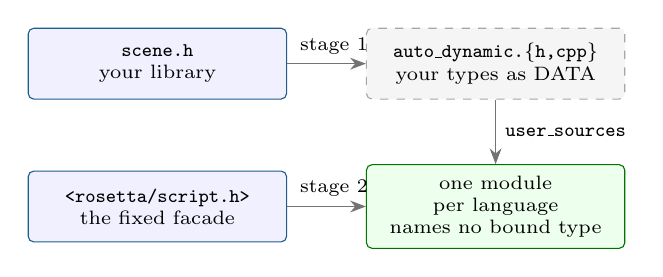
\begin{tikzpicture}[
  node distance=5mm,
  b/.style={draw,rounded corners=2pt,align=center,font=\scriptsize,inner sep=4pt,text width=30mm,minimum height=9mm},
  user/.style={b,fill=blue!6,draw=rosettablue},
  gen/.style={b,fill=black!4,draw=black!35,dashed},
  fin/.style={b,fill=green!7,draw=green!45!black},
  arr/.style={-{Stealth[length=2mm]},draw=black!55,font=\scriptsize}
]
\node[user] (h)  {\texttt{scene.h}\\\scriptsize your library};
\node[gen,right=10mm of h] (d) {\texttt{auto\_dynamic.\{h,cpp\}}\\\scriptsize your types as DATA};
\node[user,below=9mm of h] (s) {\texttt{<rosetta/script.h>}\\\scriptsize the fixed facade};
\node[fin,right=10mm of s] (m) {one module per language\\\scriptsize names no bound type};
\draw[arr] (h) -- node[above]{\ \ stage 1} (d);
\draw[arr] (s) -- node[above]{\ \ stage 2} (m);
\draw[arr] (d) -- node[right]{\texttt{user\_sources}} (m);
\end{tikzpicture}
\end{center}

By stage~2 your types are \textbf{data}, not C++. So stage~2's manifest never
names one, and the resulting module works for \emph{any} library that has been
through stage~1.

\section{Why a facade rather than binding \code{dynamic.h}}

\code{rosetta::dyn} cannot be fed to the backends as it stands. Three shapes
block it:

\begin{center}
\small
\begin{tabular}{@{}L{3.9cm}L{4.6cm}L{4.5cm}@{}}
\toprule
\textbf{In \code{dynamic.h}} & \textbf{Why it blocks} & \textbf{In
  \code{script.h}} \\
\midrule
\code{MetaField *fields; size\_t n\_fields} &
  pointer-and-count, so vector marshalling never fires &
  \code{std::vector<FieldInfo> fields()} \\
\addlinespace
\code{const MetaClass *}, \code{const TypeDesc *} &
  raw pointer to an unbound type --- the gate skips it &
  value-semantics handles \\
\addlinespace
\code{using Thunk = Any (*)(\ldots)} &
  function pointers marshal nowhere &
  ordinary \code{get} / \code{set} / \code{call} \\
\bottomrule
\end{tabular}
\end{center}

\code{<rosetta/script.h>} is that reshaping and nothing more. Each handle wraps
\textbf{one \code{const} pointer} into the tables, so binding it copies no
metadata --- the \code{.rodata} guarantee survives.

\begin{note}
Nothing in the facade is named \code{Class}, \code{Type}, \code{Object} or
\code{Method}, because those collide in the target languages
(\code{java.lang.Class}, JavaScript's \code{Object}, Lua's \code{type}). Hence
\code{ClassInfo}, \code{TypeInfo}, \code{Instance}, \code{MethodInfo}.
\end{note}

Errors come back as \code{Outcome} (an ok flag plus text), never as an
exception. Unwinding through a foreign VM's frames is how you get a crash
instead of a \code{TypeError}.

\section{The one hand-written piece}

\code{Value} is type erasure --- one C++ type standing for ``whatever the host
language just handed us''. Reflection can \emph{describe} it but cannot know
that a Python \code{float}, a Lua number and a JavaScript \code{Number} should
all become the same box. That mapping is per-language knowledge, so it is
written per language, in
\code{runtime/script/\{python,lua,node,wasm\}.h}.

Only half of each caster is per-language, though:

\begin{itemize}
  \item \textbf{Reading} a host value is irreducible --- only Python knows what
    \code{PyFloat\_Check} means.
  \item \textbf{Writing} one is the same shape everywhere, so it lives once in
    \code{rosetta::script::visit()}, and each caster supplies a sink of nine
    small methods (\code{on\_none}, \code{on\_bool}, \code{on\_int},
    \code{on\_real}, \code{on\_string}, \code{on\_enum}, \code{on\_list},
    \code{on\_object}, \code{on\_unknown}).
\end{itemize}

No two casters can drift apart on whether an enum crosses as its integer, or on
what an unclaimed type renders as.

The casters reach the generated code through \field{module\_init}'s
\field{headers}, which is the only hook that emits an \code{\#include}
\emph{after} the framework header and \emph{before} the bound classes --- exactly
the window a type caster needs. Because that list is global rather than
per-target, each file guards its whole body on a macro only its own target
defines.

\begin{warn}
One subtlety the type gate forces: \code{Value} must stay in the bound
\field{classes} list. Bindability is decided at generation time and cannot know
a caster will exist, so dropping \code{Value} would silently skip every member
that mentions it --- \code{Outcome::value}, \code{Instance::set},
\code{Instance::call}, all of it. The cost is one vestigial \code{Value} type
per module that nothing ever produces.
\end{warn}

\section{What a project has to write}

Nothing, beyond where its own files are. The binding surface is fixed, so it
ships as manifest data in \code{include/rosetta/presets/scriptable.json} and a
manifest names it:

\begin{lstlisting}[style=json]
{
    "preset": "scriptable",
    "rosetta_include": "../../include",
    "user_include": ["../lib", "../lib/bindings/dynamic"],
    "user_sources": ["../lib/bindings/dynamic/auto_dynamic.cpp"],
    "module_init": { "headers": ["auto_dynamic.h"],
                     "statements": ["bank::register_all()"] },
    "targets": ["python", "lua", "node"]
}
\end{lstlisting}

Six keys, every one about \emph{this} project. Read them against the diagram:
\field{user\_sources} is stage~1's output, and \field{module\_init} is the
\code{register\_all()} that publishes it.

\section{What it buys}

\begin{itemize}
  \item \textbf{One wrapper per language instead of one per class.} Ship the
    module once; any library that has been through the \lang{dynamic} backend
    becomes scriptable with no further code generation.
  \item \textbf{UI by query, not by codegen.} A property sheet is a walk over
    \code{fields()}: \code{doc} to tooltip, \code{range} to slider bounds,
    \code{combobox} and enumerators to a drop-down, \code{readonly} to a
    disabled row. The dispatch that a C++ property panel spends a file on is
    about ten lines of Python --- editable without recompiling anything.
  \item \textbf{Overloads come back} for the name-keyed targets. Lua, Node,
    Wasm, C\# and Java bind the first overload of a name and drop the siblings
    at generation time; through this module they do not, because
    \code{resolve()} scores the whole set at call time and can explain a
    failure.
  \item \textbf{Annotations are enforced once}, in the core, rather than
    re-implemented per backend --- a \code{range} violation comes back as the
    same message in every language.
\end{itemize}

That third point is worth dwelling on, because it is the sharpest evidence that
the IR is genuinely target-neutral. The same reflected overload set survives
into both projections; the expressiveness difference between them is
attributable entirely to \emph{when} names are resolved, not to information
lost on the way.

\begin{center}
\emph{The set of C++ members a target can express is not a property of the
target language. It is a property of when the target resolves names.}
\end{center}

\section{Running the pipeline twice}

\code{examples/plain-binding} runs it \textbf{once}: one library, one manifest,
four language bindings. That is the base case, and it is what most of this book
describes.

\code{examples/scriptable-model} runs stages 1--2 once per \emph{manifest}, and
it has two:

\begin{enumerate}
  \item \textbf{The user library to metadata.} The \lang{dynamic} backend turns
    \code{scene.h} into \code{auto\_dynamic.\{h,cpp\}} --- the same information
    the other backends spend on framework calls, emitted as plain data instead.
  \item \textbf{\code{<rosetta/script.h>} to bindings.} A second pipeline that
    binds rosetta's own reflection API, taking stage~1's output as its
    \field{user\_sources}.
\end{enumerate}

Practically: two manifests, two \code{rosetta\_gen --build} invocations, in that
order. Stage~2 must be re-run when stage~1's \emph{output location} changes ---
but not when your library's \emph{classes} change, which is the whole point.

\input{ch/16-extending}

\part{Worked examples}
\chapter{Worked examples}
\label{ch:examples}

The repository carries eighteen runnable examples. This chapter is a guide to
which one answers which question, followed by three walked through in enough
detail to copy from.

\section{The map}

\begin{center}
\small
\begin{longtable}{@{}L{5.1cm}L{8.5cm}@{}}
\toprule
\textbf{Path} & \textbf{What it shows} \\
\midrule
\endhead
\code{examples/manifest} &
  Manifest-driven generation for \code{Person}, with no class modification. The
  smallest complete case. \\
\addlinespace
\code{examples/annotate-manifest} &
  Out-of-line annotations from an external JSON file, wired by the manifest's
  \field{annotations} field. \\
\addlinespace
\code{examples/doxygen} &
  The documentation a library already has: plain Doxygen comments and default
  arguments in an untouched header become Python docstrings and keyword
  arguments, TSDoc, OpenAPI descriptions and a Markdown reference.
  Ch.~\ref{ch:documentation} \\
\addlinespace
\code{examples/geom-lib} &
  Manifest-driven bindings for a small geometry library --- nested types,
  vectors. \\
\addlinespace
\code{examples/geom-expanded} &
  Ten backends (\lang{python}, \lang{nanobind}, \lang{node}, \lang{wasm},
  \lang{qt}, \lang{qml}, \lang{csharp}, \lang{java}, \lang{lua}, \lang{julia})
  built with off-the-shelf toolchains, plus out-of-line annotations. The proof
  of Section~\ref{sec:reflection-free}. \\
\addlinespace
\code{examples/dynamic} &
  The \lang{dynamic} backend end to end: one set of generated metadata driving a
  terminal interpreter \emph{and} a Qt viewer (3-D view, property panel,
  console), neither naming a bound type. \\
\addlinespace
\code{examples/scriptable-model} &
  The two-stage pipeline of Chapter~\ref{ch:scriptable}. \\
\addlinespace
\code{examples/plain-binding} &
  One library, one manifest, four language bindings --- the base case, run
  once. \\
\addlinespace
\code{examples/trampoline-python} &
  Overriding C++ virtuals from Python: generated pybind11 trampolines from
  \code{virtual\_spec}. \\
\addlinespace
\code{examples/trampoline-node} &
  The same from JavaScript, with N-API trampolines. \\
\addlinespace
\code{examples/dynamic-lib} &
  Linking the bindings against a pre-built library --- the \field{user\_lib}
  case. \\
\addlinespace
\code{examples/moc} &
  The moc-less signals/slots/properties demo built on \code{mini\_moc.h}. \\
\addlinespace
\code{examples/docgen} &
  A reflection-driven Markdown / HTML reference generator. \\
\addlinespace
\code{examples/paraview} &
  ParaView plugin property-panel XML from an annotated \code{vtkThreshold}
  spec --- exercises every annotation feature. \\
\addlinespace
\code{examples/qt}, \code{examples/qml}, \code{examples/imgui} &
  The three inspector backends, each building a form from a reflected struct.
  \code{imgui} uses an \code{Algo.ann.json} side-car and builds with an
  off-the-shelf C++20 compiler, dependencies auto-fetched. \\
\addlinespace
\code{examples/bindings/*} &
  Hand-written reference backends --- pybind11, N-API, jlcxx, REST, embind.
  What the generator emits, written by hand, for comparison. \\
\bottomrule
\end{longtable}
\end{center}

\section{The smallest case}

\code{examples/manifest} is the one to read first. An unmodified
\code{person.h}, a manifest of ten lines, and the pipeline. It is
Chapter~\ref{ch:first} as a runnable directory.

\section{A geometry library}

\code{examples/geom-lib} is the first realistic shape: several classes, one
returning a \code{std::vector} of another, an enum, and a free function.

The two things to look at:

\begin{itemize}
  \item \textbf{Nested user types cross without being mentioned.} A
    \code{Surface} method returning \code{std::vector<Triangle>} works because
    \code{Triangle} is in \field{classes} --- not because anything says how to
    convert it.
  \item \textbf{One module per target, not one per class.} The generated
    \code{pygeom} carries \code{Model}, \code{Point}, \code{Surface},
    \code{Triangle} and \code{Kind} together.
\end{itemize}

\code{examples/geom-expanded} takes the same library and builds ten backends
with stock toolchains --- no fork anywhere in the second pass. If you want to
convince yourself (or a colleague) that the reflection-free claim is real, that
is the directory to run.

\section{The dynamic model, end to end}

\code{examples/dynamic} is the most interesting example in the repository and
the one that takes longest to appreciate.

A small scene library --- \code{Vec3}, \code{Mesh}, and a \code{Relaxer} solver
--- goes through the \lang{dynamic} backend once. Two entirely separate
consumers then drive it:

\begin{itemize}
  \item a \textbf{terminal interpreter} that lists types, gets and sets fields,
    and calls methods by name;
  \item a \textbf{Qt viewer} with a 3-D view, a property panel and a console.
\end{itemize}

Neither names a single bound type. The property panel is a walk over
\code{fields()}: \code{doc} becomes a tooltip, \code{range} becomes slider
bounds, \code{combobox} becomes a drop-down.

\subsection*{What adding a class costs}

The example's own history is the argument. Adding \code{scene::Relaxer} ---
tangential Laplacian relaxation, a genuine algorithm with tuning parameters and
one method that runs for a while --- touched three files, \emph{all of them the
library's own}:

\begin{enumerate}
  \item \code{scene.h}, to add the class;
  \item \code{Mesh.ann.json}, for one new accessor's annotation;
  \item one line of \code{manifest.json}.
\end{enumerate}

No consumer changed. Not the Qt viewer, not the interpreter, not any of the five
scriptable drivers --- yet all of them gained it: the solver appeared in the
type list, its parameters appeared in the property panel with their declared
ranges, and its method appeared as a button.

That is what ``UI by query rather than by codegen'' buys, stated as a diff.

\section{Rosetta in the wild}

Real libraries bound with rosetta, each from a single manifest and with no
hand-written wrappers:

\begin{center}
\small
\begin{tabular}{@{}L{3.2cm}L{5.0cm}L{4.6cm}@{}}
\toprule
\textbf{Project} & \textbf{Bound library} & \textbf{Targets} \\
\midrule
\code{pmp-rosetta} & PMP --- polygon mesh processing (remeshing, smoothing,
  subdivision, decimation) & Python, Node.js, WebAssembly, TypeScript \\
\addlinespace
\code{geogram-rosetta} & geogram --- geometry processing (reconstruction,
  remeshing, parameterisation, booleans) & Python, Node.js, WebAssembly,
  TypeScript, Lua \\
\addlinespace
\code{arch-rosetta} & Arch --- 3-D boundary-element geomechanics &
  Python, Node.js, WebAssembly, TypeScript \\
\addlinespace
\code{cassini-rosetta} & Cassini --- FEM geomechanical restoration, through a
  single high-level facade & Python, Node.js, WebAssembly, TypeScript \\
\addlinespace
\code{triax-rosetta} & Triax --- discrete-element triaxial compression &
  Python, Node.js, WebAssembly \\
\bottomrule
\end{tabular}
\end{center}

The geogram manifest is the best worked reference for a difficult library: it
uses \field{sequences} for \code{GEO::vector}, \field{extensions} to reach
geometry behind raw-pointer accessors, \field{signature} to pick one overload of
\code{mesh\_union}, \field{module\_init} for \code{GEO::initialize()},
\field{generated\_headers} for the configured \code{version.h}, and
\field{link\_options} for the wasm NODEFS mount --- in other words, nearly every
field in Part~II, each for a reason you can see.

\section{Extending a generated binding by hand}

Everything under \code{bindings/} is regenerated output and must never be
edited. When the generated binding misses something you need --- a helper the
walker skips, a typed-array export for a renderer --- add it in a
\textbf{separate hand-written file} compiled \emph{alongside} the generated
source, from a small build of your own that lives outside \code{bindings/}.

The binding frameworks accept several registration blocks per module, so your
file contributes a second one. Nothing generated is touched, and regenerating
never clobbers your extensions.

\begin{lstlisting}[style=cpp]
// viz_helpers.cpp -- compiled next to the generated auto_emscripten.cpp
emscripten::val mesh_positions(const pmp::SurfaceMesh &mesh);  // Float32Array
emscripten::val mesh_triangles(const pmp::SurfaceMesh &mesh);  // Uint32Array
void triangulate_mesh(pmp::SurfaceMesh &m) { pmp::triangulate(m); }

EMSCRIPTEN_BINDINGS(pmp_viz) {   // a second block; the generated one keeps its own
    emscripten::function("mesh_positions", &mesh_positions);
    emscripten::function("mesh_triangles", &mesh_triangles);
    emscripten::function("triangulate_mesh", &triangulate_mesh);
}
\end{lstlisting}

\begin{warn}
Embind is the friendliest here because it accepts any number of
\code{EMSCRIPTEN\_BINDINGS} blocks in one module. Backends with a single module
entry point --- pybind11's \code{PYBIND11\_MODULE}, N-API's
\code{NODE\_API\_MODULE} --- cannot add a second block to the \emph{same}
module. There, ship your extras as a small companion module built the same way
(it sees the same user headers and links the same library) and import both.
\end{warn}

Before reaching for this, check whether \field{extensions}
(Section~\ref{sec:extensions}) covers your case: a free function taking
\code{Cls\&} needs no build of your own and reaches every backend at once.


\appendix
\part{Reference}
\chapter{Manifest field reference}
\label{app:manifest}

Every top-level field, alphabetically. \req\ marks a required field.

\begin{center}
\small
\begin{longtable}{@{}L{3.0cm}cL{2.8cm}L{6.0cm}@{}}
\toprule
\textbf{Field} & \textbf{Req.} & \textbf{Default} & \textbf{Meaning} \\
\midrule
\endhead
\field{build\_type} & & \code{Release} &
  Default \code{CMAKE\_BUILD\_TYPE} baked into every compiled backend's
  \code{CMakeLists.txt}. \S\ref{sec:buildtype} \\
\addlinespace
\field{classes} & \req$^*$ & --- &
  The classes, structs and enums to bind. $^*$Optional when a \field{preset}
  supplies them. Ch.~\ref{ch:whattobind} \\
\addlinespace
\field{compile\_definitions} & & \code{[]} &
  Preprocessor definitions (\code{"NAME"} or \code{"NAME=VALUE"}) applied to the
  generator driver \emph{and} every compiled binding target.
  Ch.~\ref{ch:building} \\
\addlinespace
\field{cpp26\_cc} & & \code{\$\{cpp26\_root\}/}\bk\code{bin/clang} &
  C compiler of the reflection toolchain. \\
\field{cpp26\_cxx} & & \code{\$\{cpp26\_root\}/}\bk\code{bin/clang++} &
  C++ compiler of the reflection toolchain. \\
\field{cpp26\_lib} & & \code{\$\{cpp26\_root\}/lib} &
  Directory holding the fork's \code{libc++} / \code{libc++abi}. \\
\field{cpp26\_root} & & a built-in path &
  Root of the C++26 / P2996 toolchain. Moves the other three together.
  \S\ref{sec:toolchain-paths} \\
\addlinespace
\field{doc\_comments} & & \code{true} &
  Read the Doxygen documentation and default arguments already present in the
  bound headers, and carry them into every backend. \code{false} generates from
  annotations alone. Ch.~\ref{ch:documentation} \\
\addlinespace
\field{functions} & & \code{[]} &
  Free (non-member) functions to bind. \S\ref{sec:functions} \\
\addlinespace
\field{generated\_headers} & & \code{[]} &
  Headers the bound library's own build system would have produced, written
  into the generated tree and put first on the include path.
  \S\ref{sec:generatedheaders} \\
\addlinespace
\field{generator\_name} & & manifest's directory name &
  Basename of the emitted reflection driver; last-resort default for
  \field{module\_name}. \\
\addlinespace
\field{header\_dir} & & --- &
  Directory fragment prepended to every entry header.
  \S\ref{sec:shared-defaults} \\
\addlinespace
\field{interop} & & \code{[]} &
  Foreign libraries whose types the target's binding framework marshals itself
  (\code{["eigen"]}). \S\ref{sec:interop} \\
\addlinespace
\field{matrices} & & \code{[]} &
  Foreign 2-D containers that marshal as an array of row arrays.
  \S\ref{sec:matrices} \\
\addlinespace
\field{module\_init} & & --- &
  Statements the generated module runs when it \emph{loads}, plus the headers
  declaring them. \S\ref{sec:moduleinit} \\
\addlinespace
\field{module\_name} & & a preset's, else \field{generator\_name} &
  Default binding module name, used by any bare-string target. \\
\addlinespace
\field{namespace} & & --- &
  Default C++ namespace for entry names carrying no \code{::} of their own.
  \S\ref{sec:shared-defaults} \\
\addlinespace
\field{optimization} & & --- &
  Explicit optimisation flag applied after the build type's own.
  \S\ref{sec:buildtype} \\
\addlinespace
\field{out\_dir} & & --- &
  Where every target's \emph{built artifact} is copied after each build. A
  per-target \field{out\_dir} overrides it. \S\ref{sec:outdir} \\
\addlinespace
\field{out\_params} & & \code{\{\}} &
  Which parameters a method returns \emph{through a reference}, keyed
  \code{"Class::method"}. Never inferred. \S\ref{sec:outparams} \\
\addlinespace
\field{plugins} & & \code{[]} &
  Extra \code{.cpp} sources compiled into the generator driver --- a custom
  backend. Ch.~\ref{ch:extending} \\
\addlinespace
\field{preset} & & --- &
  A named JSON fragment supplying a fixed binding surface.
  Ch.~\ref{ch:presets} \\
\addlinespace
\field{rosetta\_include} & \req & --- &
  Path to rosetta's \code{include/} directory. \\
\addlinespace
\field{sequences} & & \code{[]} &
  Foreign sequence containers that marshal like \code{std::vector<T>}.
  \S\ref{sec:sequences} \\
\addlinespace
\field{targets} & \req & --- &
  The language backends to emit. Ch.~\ref{ch:targets} \\
\addlinespace
\field{user\_include} & \req & --- &
  Directory holding your class headers, or an array of directories. \\
\addlinespace
\field{user\_lib} & & --- &
  Pre-built external libraries to link the bindings against; one object or an
  array. Ch.~\ref{ch:building} \\
\addlinespace
\field{user\_sources} & & \code{[]} &
  User \code{.cpp} / \code{.c} files compiled into every binding target. Globs
  allowed. Ch.~\ref{ch:building} \\
\addlinespace
\field{variables} & & \code{[]} &
  Manifest-local variables, substituted as \code{\$NAME} / \code{\$\{NAME\}}
  into every string. \S\ref{sec:variables} \\
\addlinespace
\field{version} & & \code{0.1.0} &
  Distribution version stamped into the packaging artifacts (PEP 440).
  \S\ref{sec:wheels} \\
\bottomrule
\end{longtable}
\end{center}

Keys beginning with \code{//} are comments and are ignored everywhere,
including inside groups and entries.

\section{Class entry fields}

\begin{center}
\small
\begin{tabular}{@{}lcL{8.4cm}@{}}
\toprule
\textbf{Field} & \textbf{Req.} & \textbf{Meaning} \\
\midrule
\field{header} & \req & Filename emitted into \code{\#include}, resolved against
  \field{user\_include}. May be a glob. \\
\field{name} & & C++ type name; defaults to the header's stem. May be
  qualified. \\
\field{expose} & & The binding name. Must be a plain identifier. \\
\field{annotations} & & Path to an out-of-line annotation side-car. \\
\field{doc} & & Description for the document backends. \\
\field{extensions} & & Free functions exposed as instance methods. \\
\field{final} & & No trampoline even with public virtuals. \\
\field{exclude} & & Glob-entry only: patterns whose matches are dropped. \\
\field{entries} & & Makes this a \emph{group} rather than an entry.
  \S\ref{sec:groups} \\
\bottomrule
\end{tabular}
\end{center}

\section{Function entry fields}

\begin{center}
\small
\begin{tabular}{@{}lcL{8.4cm}@{}}
\toprule
\textbf{Field} & \textbf{Req.} & \textbf{Meaning} \\
\midrule
\field{name} & \req & Function name, optionally qualified. \\
\field{header} & \req & Header declaring it. \\
\field{doc} & & Description. \\
\field{expose} & & The binding name. \\
\field{signature} & & C++ function type of the one overload to bind. Required
  when \field{name} is overloaded, meaningless otherwise. \\
\bottomrule
\end{tabular}
\end{center}

\section{Target entry fields}

\begin{center}
\small
\begin{tabular}{@{}lcL{8.4cm}@{}}
\toprule
\textbf{Field} & \textbf{Req.} & \textbf{Meaning} \\
\midrule
\field{lang} & \req & The backend. See Appendix~\ref{app:targets}. \\
\field{name} & & Module / library name; defaults to \field{module\_name}. \\
\field{link\_options} & & Extra linker flags for this target only. \\
\field{out\_dir} & & Where this target's artifact is copied. \\
\field{python} & & Interpreter the binding is built for. \\
\field{requires\_python} & & Minimum Python version; feeds both CMake and
  \code{pyproject.toml}. \\
\field{napi\_version} & & \code{NAPI\_VERSION=} for a Node addon. \\
\field{node\_engine} & & \code{engines.node} in \code{package.json}. \\
\field{wheel} & & Build a wheel for this target on every \code{--build}.
  \lang{python} / \lang{nanobind} only --- an error elsewhere.
  \S\ref{sec:wheels} \\
\field{wheel\_dir} & & Where this target's wheels go instead of its own
  \code{dist/}. Implies \field{wheel}. \\
\bottomrule
\end{tabular}
\end{center}

A bare string in \field{targets} is shorthand for \code{\{"lang": "\ldots"\}}.

\section{\field{user\_lib} entry fields}

\begin{center}
\small
\begin{tabular}{@{}lcL{8.4cm}@{}}
\toprule
\field{name} & \req & Library base name --- the \code{space} in
  \code{libspace.dylib}. \\
\field{dir} & \req & Directory holding it; used for \code{-L} and rpath. \\
\field{link} & & \code{"shared"} (default), \code{"static"}, or
  \code{"dynamic"}. \\
\bottomrule
\end{tabular}
\end{center}

\input{ch/app-b-annotations}
\chapter{Target reference}
\label{app:targets}

\section{Every \field{lang} value}

\begin{center}
\small
\begin{longtable}{@{}lL{4.2cm}L{3.4cm}L{2.6cm}@{}}
\toprule
\textbf{\code{lang}} & \textbf{Output} & \textbf{Builds with} &
  \textbf{Overloads} \\
\midrule
\endhead
\lang{python} & pybind11 extension module & off-the-shelf compiler & all \\
\lang{nanobind} & nanobind extension module & off-the-shelf compiler & all \\
\lang{node} & N-API native addon & off-the-shelf compiler & first only \\
\lang{wasm} & Emscripten / embind module & off-the-shelf emsdk & first only \\
\lang{lua} & sol2 module, \code{require}-able & off-the-shelf compiler & first only \\
\lang{julia} & CxxWrap.jl / jlcxx module & compiler + CxxWrap.jl & all \\
\lang{csharp} & C-ABI lib + P/Invoke wrappers & compiler + .NET & first only \\
\lang{java} & C-ABI + FFM wrappers & compiler + JDK & first only \\
\lang{qt} & Qt Widgets inspector & compiler + Qt 6 & all \\
\lang{qml} & QML / QtQuick inspector & compiler + Qt 6 & first only \\
\lang{imgui} & Dear ImGui inspector app & off-the-shelf compiler & --- \\
\lang{rest} & cpp-httplib server + client & \textbf{C++26 toolchain} & first only \\
\lang{openapi} & OpenAPI 3.1 specification & text output & --- \\
\lang{json} & nlohmann (de)serialisation & \textbf{C++26 toolchain} & --- \\
\lang{typescript} & ambient \code{.d.ts} declarations & text output & first only \\
\lang{markdown} & API reference document & text output & --- \\
\lang{html} & styled API reference page & text output & --- \\
\lang{paraview} & Server Manager plugin XML & text output & --- \\
\lang{dynamic} & the IR as runtime data & off-the-shelf compiler & all, at
  call time \\
\bottomrule
\end{longtable}
\end{center}

Each name also accepts a deprecated \code{-expanded} spelling resolving to the
same backend.

\section{Feature support}

Which manifest features reach which backend. A blank cell means the backend
ignores the field rather than failing.

\begin{center}
\small
\begin{longtable}{@{}lccccc@{}}
\toprule
\textbf{\code{lang}} & \field{module\_init} & \field{out\_dir} &
  \field{extensions} & \field{sequences} & \field{out\_params} \\
\midrule
\endhead
\lang{python}     & \yes & \yes & \yes & \yes & \yes \\
\lang{nanobind}   & \yes & \yes & \yes & \yes & \yes \\
\lang{node}       & \yes & \yes & \yes & \yes & \yes \\
\lang{wasm}       & \yes & \yes & \yes & \yes & \yes \\
\lang{lua}        & \yes & \yes &      & \yes & \yes \\
\lang{julia}      & \yes & \yes &      &      &      \\
\lang{csharp}     &      &      &      &      &      \\
\lang{java}       &      &      &      &      &      \\
\lang{qt}         &      &      &      &      &      \\
\lang{qml}        &      &      &      &      &      \\
\lang{imgui}      &      &      &      &      &      \\
\lang{rest}       &      &      &      &      &      \\
\lang{typescript} &      &      & \yes & \yes & \yes \\
\lang{markdown}   &      &      & \yes &      &      \\
\lang{html}       &      &      & \yes &      &      \\
\bottomrule
\end{longtable}
\end{center}

\section{Documentation output}

Where each backend puts the documentation, parameter names and default
arguments harvested from your headers (chapter~\ref{ch:documentation}). A dash
means the target has nowhere to put it, not that the data is missing from the
IR.

\begin{center}
\small
\begin{longtable}{@{}lL{5.6cm}L{5.0cm}@{}}
\toprule
\textbf{\code{lang}} & \textbf{Documentation lands as} &
  \textbf{Names \& defaults} \\
\midrule
\endhead
\lang{python} \lang{nanobind} & docstring, with \code{Args:} /
  \code{Returns:} sections; the class comment is the type's docstring &
  \code{py::arg} / \code{nb::arg} keyword arguments; real Python defaults
  (see the import-time rule) \\
\addlinespace
\lang{typescript} & TSDoc block: prose, \code{@param}, \code{@returns} &
  names in the signature; a defaulted parameter is \code{optional?} \\
\addlinespace
\lang{markdown} \lang{html} & prose, a list of documented arguments, a
  \emph{Returns} line & \code{name: type = default} in the signature \\
\addlinespace
\lang{openapi} & operation \code{description}; per-argument
  \code{description} & argument \code{title}, and \code{default} where the
  value is expressible in JSON \\
\addlinespace
\lang{csharp} & \code{/// <summary>} XML doc & names in the wrapper
  signature (keyword-guarded) \\
\addlinespace
\lang{java} & Javadoc block & names in the wrapper signature
  (keyword-guarded) \\
\addlinespace
\lang{qt} \lang{qml} \lang{imgui} & a field's tooltip & the name labels the
  argument box \\
\addlinespace
\lang{dynamic} & text in the emitted \code{MetaClass} tables & names in the
  parameter tables \\
\addlinespace
\lang{node} \lang{wasm} \lang{lua} \lang{julia} & --- (no docstring slot;
  pair with \lang{typescript}) & --- (the wrappers spell positional locals) \\
\addlinespace
\lang{rest} & --- (the spec is \lang{openapi}'s job) & names in the
  browser client's field placeholders \\
\addlinespace
\lang{json} \lang{paraview} & --- & --- \\
\bottomrule
\end{longtable}
\end{center}

\section{Packaging}

Only two backends emit a \code{make\_wheel.py}, so only those two accept the
per-target \field{wheel} / \field{wheel\_dir} (Section~\ref{sec:wheels}); the
field is an error on any other \field{lang}.

\begin{center}
\small
\begin{tabular}{@{}lL{9.4cm}@{}}
\toprule
\lang{python} & One wheel per CPython version --- pybind11 has no stable-ABI
  mode. Covering several means running \code{make\_wheel.py} once per
  interpreter. \\
\lang{nanobind} & One \code{abi3} wheel covering every CPython 3.12+; below
  3.12, tagged for the exact interpreter that built it. \\
every other & No packaging step. \\
\bottomrule
\end{tabular}
\end{center}

\section{Interop and foreign types}

\begin{center}
\small
\begin{tabular}{@{}lL{9.4cm}@{}}
\toprule
\textbf{\code{lang}} & \textbf{\field{interop}: \code{["eigen"]}} \\
\midrule
\lang{python} & native numpy, through \code{<pybind11/eigen.h>} \\
\lang{nanobind} & native numpy, through \code{<nanobind/eigen/dense.h>}
  (dense only) \\
every other & skips the member --- register the concrete type under
  \field{sequences} / \field{matrices} to give them a flat array \\
\bottomrule
\end{tabular}
\end{center}

\begin{center}
\small
\begin{tabular}{@{}lL{4.4cm}L{4.6cm}@{}}
\toprule
\textbf{\code{lang}} & \textbf{\code{std::filesystem::path}} &
  \textbf{\code{std::shared\_ptr<T>} returned} \\
\midrule
\lang{python} & native (\code{os.PathLike} in, \code{pathlib.Path} out) &
  \code{py::class\_<T, shared\_ptr<T>>} \\
\lang{nanobind} & native & native \\
\lang{wasm} & string, via a copy adapter & \code{.smart\_ptr<\ldots>} on the
  class \\
\lang{lua} & string, via a copy adapter & native (sol2) \\
\lang{node} & string, via a copy adapter & the JS object adopts the pointer;
  untrampolined pointees only \\
\lang{typescript} & \code{string} & the pointee type \\
\bottomrule
\end{tabular}
\end{center}

A \code{shared\_ptr<T>} \emph{parameter} is skipped everywhere --- take
\code{const T\&}.

\section{Build shapes for \code{--build}}

\begin{center}
\small
\begin{tabular}{@{}L{6.0cm}L{7.0cm}@{}}
\toprule
\textbf{Backend} & \textbf{Build} \\
\midrule
\lang{python}, \lang{nanobind}, \lang{rest}, \lang{json}, \lang{lua},
  \lang{imgui} & plain \code{cmake} configure + build \\
\lang{node} & \code{npm install} + \code{npm run build} \\
\lang{wasm} & \code{emcmake cmake} + \code{cmake --build} \\
\lang{julia} & \code{cmake} (locates JlCxx by running \code{julia}) \\
\lang{csharp} & \code{cmake}, then \code{dotnet build} \\
\lang{java} & \code{cmake}, then \code{mvn package} \\
\lang{qt}, \lang{qml} & \code{cmake} with \code{-DQT\_DIR} \\
\lang{markdown}, \lang{html}, \lang{typescript}, \lang{openapi},
  \lang{paraview} & nothing to compile \\
\bottomrule
\end{tabular}
\end{center}

A missing toolchain is a \emph{skip with a note}, not a failure. A missing
\code{dotnet} or \code{mvn} downgrades its backend to ``OK (native only)''.

\section{External requirements}

\begin{center}
\small
\begin{tabular}{@{}lL{9.2cm}@{}}
\toprule
\lang{python} & pybind11 (\code{pip install pybind11}) \\
\lang{nanobind} & nanobind; wheels are \code{abi3} on Python 3.12+ \\
\lang{node} & npm, and \code{cmake-js} \\
\lang{wasm} & an activated emsdk \\
\lang{lua} & Lua 5.1--5.4 or LuaJIT --- \textbf{not} 5.5, which sol2 does not
  support yet. sol2 itself is fetched at configure time \\
\lang{julia} & CxxWrap.jl; the build runs \code{julia} to locate JlCxx \\
\lang{csharp} & a .NET SDK \\
\lang{java} & a JDK with the FFM API \\
\lang{qt}, \lang{qml} & Qt 6 --- but no \code{moc} on the generated code \\
\lang{imgui} & nothing; GLFW and OpenGL3 are auto-fetched \\
\lang{rest} & cpp-httplib and nlohmann/json, fetched on first configure, plus
  the C++26 toolchain \\
\bottomrule
\end{tabular}
\end{center}

\input{ch/app-d-troubleshooting}

\end{document}
